\documentclass[11pt]{article}
\usepackage[T1]{fontenc}
\usepackage{lmodern}
\usepackage[margin=1in]{geometry}
\usepackage{amsmath,amssymb,amsthm,mathtools,bm}
\usepackage{microtype}
\usepackage{enumitem}
\usepackage{booktabs}
\usepackage{needspace}
\usepackage{tikz}
\usetikzlibrary{arrows.meta,calc,patterns,positioning}
\usepackage[colorlinks=true,linkcolor=black,citecolor=black,urlcolor=blue]{hyperref}
\hypersetup{pdftitle={Nonuniqueness for Bounded Measurable Scalar Conductivities in Three Dimensions},pdfauthor={OpenAI}}
\setlength{\emergencystretch}{2em}
\clubpenalty=10000
\widowpenalty=10000
\numberwithin{equation}{section}
\newtheorem{theorem}{Theorem}[section]
\newtheorem{lemma}[theorem]{Lemma}
\newtheorem{proposition}[theorem]{Proposition}
\newtheorem{corollary}[theorem]{Corollary}
\theoremstyle{definition}
\newtheorem{definition}[theorem]{Definition}
\theoremstyle{remark}
\newtheorem{remark}[theorem]{Remark}
\newcommand{\R}{\mathbb R}
\newcommand{\T}{\mathbb T}
\newcommand{\N}{\mathbb N}
\newcommand{\eps}{\varepsilon}
\newcommand{\dd}{\,\mathrm d}
\newcommand{\Id}{I}
\DeclareMathOperator{\tr}{tr}
\DeclareMathOperator{\supp}{supp}
\DeclareMathOperator{\dist}{dist}
\DeclareMathOperator{\Div}{div}
\DeclareMathOperator{\diag}{diag}
\DeclareMathOperator{\rank}{rank}
\newcommand{\norm}[1]{\left\lVert #1\right\rVert}
\newcommand{\abs}[1]{\left\lvert #1\right\rvert}
\newcommand{\ip}[2]{\left\langle #1,#2\right\rangle}

\title{Nonuniqueness for Bounded Measurable Scalar\\ Conductivities in Three Dimensions}
\author{OpenAI}
\date{September 23, 2026}

\begin{document}
\maketitle
\begin{abstract}
We construct two distinct uniformly positive bounded measurable scalar
conductivities on a ball in $\R^3$ with the same full
Dirichlet-to-Neumann operator. Both conductivities equal one near the
boundary. This gives nonuniqueness in the scalar Calder\'on problem at
bounded measurable regularity.
\end{abstract}

\section{Introduction}\label{sec:introduction}

Let $\Omega\subset\R^n$ be a bounded connected Lipschitz domain and
let $\gamma\in L^\infty(\Omega;\R)$ satisfy
$0<c\leq\gamma\leq C<\infty$ almost everywhere. For
$f\in H^{1/2}(\partial\Omega)$, let $u_f\in H^1(\Omega)$ be the
unique function of trace $f$ satisfying
\begin{equation}\label{eq:weak-model}
 \int_\Omega\gamma\nabla u_f\cdot\nabla\varphi\dd x=0
 \qquad(\varphi\in H^1_0(\Omega)).
\end{equation}
Its full weak Dirichlet-to-Neumann operator is defined by
\begin{equation}\label{eq:dn-definition}
 \ip{\Lambda_\gamma f}{g}
 =\int_\Omega\gamma\nabla u_f\cdot\nabla v\dd x,
 \qquad \operatorname{Tr}v=g.
\end{equation}
Equation~\eqref{eq:weak-model} makes this independent of the
extension $v$. Our result concerns this entire operator on the usual
trace space, at zero frequency.
The inverse problem asks whether the boundary response to every applied
voltage determines the conductivity inside the domain.

\begin{theorem}\label{thm:main}
There exist real scalar functions $\gamma_0,\gamma_1\in
L^\infty(B(0,3);\R)$ and constants $0<c<C<\infty$ such that
\begin{enumerate}[label=\textup{(\roman*)},itemsep=2pt]
\item $c\leq\gamma_j\leq C$ almost everywhere, for $j=0,1$;
\item both conductivities equal $1$ in a neighborhood of the boundary;
\item $\abs{\{x:\gamma_0(x)\ne\gamma_1(x)\}}>0$;
\item $\Lambda_{\gamma_0}=\Lambda_{\gamma_1}$ as bounded operators
from $H^{1/2}(\partial B(0,3))$ to $H^{-1/2}(\partial B(0,3))$.
\end{enumerate}
\end{theorem}

Thus the scalar Calder\'on uniqueness assertion with only bounded
measurability and uniform positivity has a negative resolution, already
in dimension three. In particular, the assertion quantified over every
$n\geq3$ is false. The theorem imposes no derivative regularity and
does not prescribe the contrast $C/c$ or assert a construction in every
higher dimension.

\begin{corollary}[Localized nonuniqueness]\label{cor:localized}
Let $c,C$ be the constants in Theorem~\ref{thm:main}.
For every bounded connected Lipschitz domain $\Omega\subset\R^3$
and every finite family of pairwise disjoint balls
$B_1,\ldots,B_m\Subset\Omega$, $m\geq1$, there are $2^m$
pairwise distinct real scalar conductivities
$\gamma_\varepsilon\in L^\infty(\Omega)$, indexed by
$\varepsilon\in\{0,1\}^m$, such that
\[
 c\leq\gamma_\varepsilon\leq C\quad\text{almost everywhere},
 \qquad
 \gamma_\varepsilon=1\quad\text{on }
 \Omega\setminus\bigcup_{i=1}^m B_i,
\]
and all their full weak Dirichlet-to-Neumann operators from
$H^{1/2}(\partial\Omega)$ to $H^{-1/2}(\partial\Omega)$ agree.
Distinct conductivities differ on a set of positive measure.
\end{corollary}

The proof, given after the main construction, copies the pair into
smaller separated balls and minimizes energy over their interface
traces. It does not require the common response to be that of the
constant conductivity one.

\paragraph{Regularity and related constructions.}
Calder\'on posed the determination problem for bounded measurable real
scalar conductivities bounded away from zero, and proved injectivity of
its linearization at constant conductivities~\cite{Calderon}.
For the nonlinear problem in dimensions at least three, Sylvester and
Uhlmann established full-boundary uniqueness for smooth scalar
conductivities~\cite{SylvesterUhlmann}. Later results reach lower
regularity. Haberman proves uniqueness for uniformly elliptic
$W^{1,n}$ conductivities in dimensions three and four
\cite[Theorem~1.1]{Haberman}; Caro and Rogers prove it for positive
Lipschitz conductivities in every dimension at least three
\cite[Theorem~1.1]{CaroRogers}. In the plane, Astala and P\"aiv\"arinta
prove uniqueness for bounded measurable uniformly positive scalar
conductivities on bounded simply connected domains
\cite[Theorem~1]{AstalaPaivarinta}. Theorem~\ref{thm:main} concerns the
three-dimensional measurable class, without the derivative hypotheses
of the cited higher-dimensional results.

The companion scalar corollary proves uniqueness for strictly positive
conductivities smooth up to the boundary of a bounded connected smooth
domain in $\mathbb R^n$, $n\ge3$, with Dirichlet inputs supported in any
nonempty relatively open boundary patch and conductivity flux observed on
that same patch~\cite[Corollary~1.3]{OpenAISmoothPatch2026}.

For rough matrix-valued conductivities, nonunique continuation provides
a route to inverse nonuniqueness. Daud\'e, Kamran, and Nicoleau
\cite[Theorem~1 and Proposition~1.2]{DaudeKamranNicoleau}
combine Miller's construction~\cite{Miller} with a conformal change
to obtain anisotropic counterexamples with partial boundary data.
Their full-boundary obstruction
\cite[Remark~1.3]{DaudeKamranNicoleau} also explains a difficulty
for the present problem: a weakly harmonic factor with constant full
boundary trace is itself constant by the energy identity. The factor
used below has a nonzero interior source, subject to a more specific
annihilation identity.

Scalar approximation of matrix conductivities raises a separate
issue. Marino and Spagnolo~\cite{MarinoSpagnolo} establish isotropic
density in the sense of $G$-convergence. Rondi, using an example
communicated by Giovanni Alessandrini, makes the distinction between
such approximation and exact boundary-map realization explicit
\cite[Proposition~2.2, Theorem~4.3, and Example~4.4]{Rondi}.
On the unit disc, a constant matrix $\diag(a,b)$ with $a,b>0$ and
$a\ne b$ is an $H$-limit of scalar coefficients, with ellipticity
bounds allowed to widen, but has no bounded uniformly positive scalar
representative with the same full boundary map. The scalarization used
here preserves exact responses to two prescribed inputs; a further
argument is needed to reach every input.

\paragraph{From a scalar block to the full operator.}
The construction in Section~\ref{sec:nonuniqueness} takes
$\Omega=B(0,3)$ and nests scaled copies of a scalar block with one
parent and two child boundary tori. Each torus carries a specified
probability measure. The block can realize every current triple
$p=(p_0,p_-,p_+)$ in the plane $p_0+p_-+p_+=0$, with flux equal to
$p_i$ times the corresponding measure. After its parent voltage is
normalized to zero, the potential extends by constants into the
adjacent regions as an admissible compactly supported test for any
global $\gamma$-harmonic function $u$.
Reciprocity therefore gives
\[
 p_0m_0(u)+p_-m_-(u)+p_+m_+(u)=0
 \qquad(p_0+p_-+p_+=0),
\]
where $m_i(u)$ is the trace average on the indicated surface. The
three averages are equal because their vector is orthogonal to the
zero-sum plane. Iterating through the nested blocks gives one common
average $u_*$ on every cell surface, for every global harmonic $u$.

Signed currents propagated through the cells produce a nonzero
$w\in H^1_0(\Omega)\cap L^\infty(\Omega)$ supported away from the
outer boundary. The common averages and shrinking cell diameters imply
that its source satisfies
\[
 \int_\Omega\gamma\nabla w\cdot
       \nabla\bigl((u-u_*)\phi\bigr)\dd x=0
 \qquad\bigl(\phi\in C_c^\infty(\Omega)\bigr)
\]
for every bounded weakly $\gamma$-harmonic $u$. The source is not zero;
it vanishes on these particular products. This is the property used
to change the conductivity.

Choose a sufficiently small nonzero $\delta$ so that $\rho=1+\delta w$
is positive, and set
\[
 \widetilde\gamma=\rho^2\gamma,
 \qquad
 \widetilde u=u_*+\frac{u-u_*}{\rho}.
\]
The corresponding flux is
\[
 \widetilde\gamma\nabla\widetilde u
 =\rho\gamma\nabla u-(u-u_*)\gamma\nabla\rho.
\]
The product identity, together with the original weak equation tested
against $\rho\phi$, makes this flux divergence free. In the outer collar
$\rho=1$, so the transformed solution and flux agree with the original
ones. Smooth boundary voltages have bounded harmonic extensions, so
their boundary responses agree; boundedness and density then give
equality of the full operators on $H^{1/2}(\partial\Omega)$. The
nonzero potential makes the two positive conductivities distinct. Thus
the source identity, applied to every bounded harmonic function, is the
step from the block's finite family of controlled inputs to the full
inverse problem.

\paragraph{Constructing the scalar block.}
Section~\ref{sec:scalarization} proves an exact finite-field
scalarization theorem. Under the stated local smoothness and rank
conditions, it replaces a uniformly elliptic symmetric tensor by one
bounded positive scalar coefficient while preserving the voltage trace
and the entire normal-flux functional of each of two designated
solutions. Here ``finite-field'' refers to the number of chosen inputs,
not to a finite-dimensional observation of each response.

The product scalar leaves and successive coordinate joins have a
classical antecedent in the isotropic approximation of Marino and
Spagnolo~\cite[\S3]{MarinoSpagnolo}. The localized flux waves use the
polynomial potential method of Rai\textcommabelow{t}\u a
\cite[Theorem~1 and \S2]{Raita}; the proof gives the explicit
formula for a surjective symbol and the coupled construction required
here. Together with a synchronized coordinate change and a small
symmetric tensor correction, these waves produce successive perturbations
satisfying the exact equations and preserving both boundary responses.
A Baire continuity-point argument then selects a strong limit satisfying
one scalar constitutive relation for both fields. This uses
the method developed by Kirchheim~\cite{Kirchheim} and adapted to
elliptic equations by Astala, Faraco, and Sz\'ekelyhidi
\cite[Lemmas~3.7--3.8]{AstalaFaracoSzekelyhidi}. These precedents
supply methods; the simultaneous Cauchy-pair conclusion is proved in
Section~\ref{sec:scalarization}.

Section~\ref{sec:block} supplies the tensor and the two designated
fields. It builds a block with one parent and two child boundary tori,
and makes both fields affine in the normal coordinate at all three
ends. The construction corrects small residuals across rank-one walls,
then transfers a decaying mode through successively doubled angular
frequencies until it vanishes at finite distance. The two resulting
current vectors span the zero-sum plane. After scalarization, those two
responses and the constant solution cover every separately constant
voltage vector on the three boundary components. This is precisely the
block property used to force the common surface averages above.

\section{Weak equations and changes of variables}\label{sec:prelim}

We use real functions throughout; complex trace spaces, if desired,
follow by complex linear extension. Let $U\subset\R^3$ be bounded
and Lipschitz. A tensor is a measurable symmetric matrix $A$ with
$a\Id\leq A\leq b\Id$ almost everywhere, where $0<a<b<\infty$.
The weak equation is $\Div(A\nabla u)=0$, interpreted as in
Equation~\eqref{eq:weak-model}. The trace theorem, the zero-trace
Poincar\'e inequality, and coercivity give existence and uniqueness for
each trace. A weak solution minimizes its energy among functions of
that trace: if $h\in H^1_0(U)$, then
\begin{equation}\label{eq:energy-minimum}
 \int_U A\nabla(u+h)\cdot\nabla(u+h)
 =\int_U A\nabla u\cdot\nabla u+
   \int_U A\nabla h\cdot\nabla h.
\end{equation}
Testing positive and negative truncations gives the usual maximum
bound when the trace is bounded. These facts require no derivative
of $A$.

For a divergence-free $F\in L^2(U;\R^3)$, its normal flux is the
continuous functional
\begin{equation}\label{eq:normal-functional}
 \ip{F\cdot\nu}{\operatorname{Tr}v}
 :=\int_U F\cdot\nabla v\dd x\qquad(v\in H^1(U)).
\end{equation}
It is well defined because the integral vanishes for zero-trace
functions. A Cauchy pair consists of $\operatorname{Tr}u$ and this
functional for $F=A\nabla u$. This convention also fixes all signs
when a function on a block is extended by constants across its
boundary components.

We will use that matching traces glue $H^1$ functions across Lipschitz
interfaces. Also $H^1\cap L^\infty$ is an algebra, with the ordinary
weak product rule; Lipschitz compositions on the range of a function
obey the weak chain rule. In particular truncation commutes with the
trace, so the trace of a bounded $H^1$ function inherits its bounds.
All interfaces used for these operations are finite unions of
Lipschitz pieces; infinite constructions are passed to the limit in
$H^1$ explicitly.

For later reference, let $x=X(y)$ be a bi-Lipschitz change of variables
that is smooth with nonsingular derivative on open pieces covering
almost every point. Write $J=DX$ and set, at $x=X(y)$,
\begin{equation}\label{eq:pushforward}
 \widehat u(x)=u(y),\qquad
 \widehat A(x)=\frac{J A(y)J^t}{\abs{\det J}},\qquad
 \widehat F(x)=\frac{J F(y)}{\abs{\det J}}.
\end{equation}
Then $\nabla\widehat u=J^{-t}\nabla u$, and change of variables gives
\begin{equation}\label{eq:pushforward-test}
 \int_{X(U)}\widehat F\cdot\nabla\phi\dd x
 =\int_U F\cdot\nabla(\phi\circ X)\dd y.
\end{equation}
Thus divergence-free fluxes remain divergence free, and the tensor
rule preserves the weak energy pairing. A right-hand side transforms
as a density: $\widehat r(X(y))=r(y)/\abs{\det J(y)}$.
Symmetry and uniform ellipticity persist, with bounds depending on
the bi-Lipschitz constants. If $X$ is the identity outside an interior
box, both Cauchy data are unchanged. We will apply the same rules to
potential coordinates and to the piecewise smooth physical collars.

\section{Exact scalarization of two Cauchy pairs}
\label{sec:scalarization}

This section replaces a matrix conductivity by a scalar one while
preserving two specified Cauchy pairs exactly. This is a finite-field
statement: it preserves the full flux response to each of two prescribed
voltage inputs, not the matrix conductivity's full
Dirichlet-to-Neumann operator. Classical isotropic approximation in
$G$-convergence provides useful historical context
\cite{MarinoSpagnolo}, but no homogenization result is used below.
The exact boundary data follow from localized perturbations and a
strong limit selected by the Baire theorem.
The continuity-point method follows the Baire-category framework for
differential inclusions developed by Kirchheim~\cite{Kirchheim} and
used for elliptic equations by Astala, Faraco, and
Sz\'ekelyhidi~\cite[Lemmas~3.7--3.8]{AstalaFaracoSzekelyhidi}.
We give the complete
localized construction and limiting argument for the simultaneous
Cauchy-pair constraints needed here.

\begin{theorem}[Exact finite-field scalarization]
\label{thm:scalarization}
Let $U\subset\R^3$ be a bounded Lipschitz domain. Let $A$ be a
measurable symmetric matrix field satisfying
\[
 c_0\Id\leq A\leq C_0\Id\qquad\text{almost everywhere in }U,
 \qquad 0<c_0\leq C_0<\infty.
\]
Suppose the real-valued potentials $u_1,u_2\in H^1(U)$ satisfy
$\Div(A\nabla u_j)=0$. Assume that there is an open cover of a
full-measure subset of $U$ on whose members $A,u_1,u_2$ are smooth
and have the following local rank property. On each member, a fixed
subset of the potentials has everywhere independent gradients, and
every remaining potential is a constant affine combination of that
subset. The subset may have zero, one, or two elements; a zero-element
subset means that both potentials are constant there.

There exist constants $0<a<b<\infty$, a measurable scalar
$a\leq\gamma\leq b$, and $v_1,v_2\in H^1(U)$ such that
\begin{align}
 \Div(\gamma\nabla v_j)&=0,
 &v_j-u_j&\in H^1_0(U), \label{sc:conclusion-equations}\\
 \int_U\gamma\nabla v_j\cdot\nabla\psi\,\dd x
 &=\int_U A\nabla u_j\cdot\nabla\psi\,\dd x
 &&\text{for every }\psi\in H^1(U). \label{sc:conclusion-flux}
\end{align}
The bounds $a,b$ may be chosen using only $c_0,C_0$.
\end{theorem}

We use the Euclidean norm for vectors and the Frobenius norm for
matrices. Write $\mathrm{Sym}_3$ for the vector space of real symmetric
$3\times3$ matrices, with this norm. Gradient and flux matrices have
their fields as columns.
In particular, $E^tF$ is the matrix of their pointwise pairings.
The proof will not require a positive lower bound on the independent
gradients throughout $U$: such bounds are used only on individual
compactly contained coordinate boxes.

\subsection{An open class of finite laminates}

For positive triples $\alpha,\beta\in(0,\infty)^3$, a coordinate
direction $i$, and $0\leq\theta\leq1$, define their coordinate join
$J_i(\theta;\alpha,\beta)$ by
\begin{equation}
 \label{sc:join}
 [J_i]_i=\left(\frac{\theta}{\alpha_i}
                  +\frac{1-\theta}{\beta_i}\right)^{-1},
 \qquad
 [J_i]_\ell=\theta\alpha_\ell+(1-\theta)\beta_\ell
 \quad(\ell\ne i).
\end{equation}
Fix $0<a<b$. Let $\mathcal G^{\mathrm{diag}}$ consist of the
triples obtainable by a finite tree of these joins, starting from
scalar triples $(s,s,s)$ with $a<s<b$. A tree is evaluated in one
fixed coordinate frame. Let $\mathcal G$ be its spectral extension:
\[
 \mathcal G=
 \{Q\diag(\alpha)Q^t:
       Q\text{ orthogonal},\ \alpha\in\mathcal G^{\mathrm{diag}}\}.
\]
In particular, every matrix in $\mathcal G$ lies strictly between
$a\Id$ and $b\Id$.

\begin{lemma}[Openness and coverage]
\label{sc:open-class}
The set $\mathcal G^{\mathrm{diag}}$ is open in $\R^3$, and
$\mathcal G$ is open in $\mathrm{Sym}_3$.
Every joining path in a representing tree lies in $\mathcal G$.
Given $c_0,C_0$, the numbers $a,b$ can be chosen so that every
symmetric matrix with spectrum in $[c_0,C_0]$ belongs to
$\mathcal G$.
\end{lemma}

\begin{proof}
The product construction below is related to the diagonal
approximation in Marino and Spagnolo~\cite[Section~3]{MarinoSpagnolo};
we use its elementary coordinate-join arithmetic directly.
First we show that each scalar triple strictly between the endpoints
is interior. Given a nearby positive triple $(\alpha_1,\alpha_2,
\alpha_3)$, choose $M>\max_i\alpha_i$ and set
\[
 d_i=\sqrt{1-\alpha_i/M}.
\]
Let $t_i$ independently take the two values $1-d_i,1+d_i$ with
equal weights. Its arithmetic mean is one and its harmonic mean is
$1-d_i^2=\alpha_i/M$. Start with the eight scalar leaves
\begin{equation}
 \label{sc:product-leaves}
 M t_1t_2t_3\Id.
\end{equation}
Joining the $t_1$ pairs in direction 1 gives the diagonal triple
\[
 (\alpha_1t_2t_3,Mt_2t_3,Mt_2t_3).
\]
Joining the $t_2$ pairs in direction 2 gives
$(\alpha_1t_3,\alpha_2t_3,Mt_3)$, and the direction-3 joins give
$(\alpha_1,\alpha_2,\alpha_3)$. If the target tends to $(s,s,s)$,
choose $M$ tending to $s$ from above. Every leaf then tends to $s$,
so all leaves lie in $(a,b)$ for sufficiently close targets.

Interior propagates through any nontrivial join. With the other
child and a weight $0<\theta<1$ fixed, the derivative of the join
in its first child is diagonal, with entries $\theta$ in the
tangential positions and $\theta[J_i]_i^2/\alpha_i^2>0$ in the
normal position. It is invertible. The inverse function theorem,
applied successively up a finite tree, proves openness in diagonal
variables. Zero-weight joins can be removed. The diagonal class is
permutation invariant; continuity of ordered eigenvalues now proves
that its spectral extension is open, including at repeated
eigenvalues. Varying the weight of an existing join simply supplies
another finite tree with the same children, so its entire path,
including its endpoints, stays in $\mathcal G$.

For uniform coverage, take $M=2C_0$ in
Equation~\eqref{sc:product-leaves}. For targets in $[c_0,C_0]^3$,
all factors lie between
\[
 \ell=1-\sqrt{1-c_0/(2C_0)}>0
 \quad\text{and}\quad 2.
\]
All leaves therefore lie in $[M\ell^3,8M]$. For example,
$a=M\ell^3/2$ and $b=16M$ put them strictly inside the leaf
interval, uniformly for the entire required spectral range.
\end{proof}

Fix these $a,b$ for the rest of the proof. The distance of a joining
path from $\mathrm{Sym}_3\setminus\mathcal G$ can depend on the path,
but every fixed path is compact in the open set $\mathcal G$ and hence
has positive such distance. All corrections below are symmetric and
will respect that distance. Thus every corrected matrix remains in
the same $\mathcal G$, and the global bounds $a,b$ never deteriorate.

We now fix the equations and boundary data that every intermediate
field must preserve. Write $A^{\rm in},u_1^{\rm in},u_2^{\rm in}$
for the data of Theorem~\ref{thm:scalarization}, and put
$F_j^{\rm in}=A^{\rm in}\nabla u_j^{\rm in}$.

\begin{definition}[Subsolution]\label{sc:subsolution}
A subsolution consists of a measurable symmetric matrix $A$, two
potentials $u_1,u_2\in H^1(U)$, and the column matrices
\[
 E=(\nabla u_1,\nabla u_2),\qquad F=AE,
\]
such that $A\in\mathcal G$ almost everywhere and, for $j=1,2$,
\begin{align*}
 u_j-u_j^{\rm in}&\in H^1_0(U),& \Div F_j&=0,\\
 \int_U F_j\cdot\nabla\psi\,\dd x
 &=\int_U F_j^{\rm in}\cdot\nabla\psi\,\dd x
 &&\text{for every }\psi\in H^1(U).
\end{align*}
It must also have an open cover of a full-measure subset of $U$ on
which $A,u_1,u_2$ are smooth and have the local rank property in
Theorem~\ref{thm:scalarization}: on each member one fixed subset of
the potentials has independent gradients, and every remaining potential
is a constant affine combination of those potentials.
\end{definition}

The original fields are a subsolution by Lemma~\ref{sc:open-class}.
The construction will change the matrix and interior fields while keeping
the equations and the two entire boundary responses in this definition.

\subsection{A split in preliminary coordinates}

We first compute the states to be realized by a local perturbation.
A divergence-free flux wave with the potentials held fixed can mix the
tangential entries of a coordinate join. The normal entry requires its
harmonic mean instead. We obtain both at once by coupling the flux wave
to a normal change of variables; the following states describe that
coupling before localization.
Freeze a parent matrix $A_0$ and its two diagonal children $A^+$,
$A^-$ in a common orthonormal frame. Let the layering direction be
the unit vector $d$, and let the physical fractions be
$\theta_+,\theta_->0$, with sum one. A trivial join needs no
perturbation. Subscripts $d$ and $T$ denote the normal scalar entry
and tangential diagonal block. Set
\begin{equation}
 \label{sc:preliminary-states}
 q_s=\frac{A_d^s}{(A_0)_d},\qquad
 B_d^s=(A_0)_d,\qquad B_T^s=q_s A_T^s,
 \qquad \eta_s=\frac{\theta_s}{q_s},
 \quad s\in\{+,-\}.
\end{equation}
The normal harmonic-mean formula and the tangential arithmetic-mean
formula give
\begin{equation}
 \label{sc:means}
 \eta_++\eta_-=1,\qquad
 \eta_+q_++\eta_-q_-=1,\qquad
 \eta_+B^++\eta_-B^-=A_0.
\end{equation}
The fractions $\eta_s$, not $\theta_s$, are used before the
coordinate change.

Put $\Delta B=B^+-B^-$ and $\Delta q=q_+-q_-$. A scalar parameter
$z\in[-\eta_+,\eta_-]$ describes the segment
\begin{equation}
 \label{sc:synchronized-segment}
 B(z)=A_0+z\Delta B,\qquad q(z)=1+z\Delta q.
\end{equation}
Its endpoints are the two states in
Equation~\eqref{sc:preliminary-states}; its barycenter is $z=0$.
The normal stretch
$L(z)=\Id+(q(z)-1)d\otimes d$ pushes $B(z)$ forward to
\begin{equation}
 \label{sc:predicted-matrix}
 C(z)=\frac{L(z)B(z)L(z)^t}{\det L(z)}
      =\diag\bigl(q(z)(A_0)_d,\ B_T(z)/q(z)\bigr)
\end{equation}
in the chosen frame. This entire path is the original coordinate
joining path, with changed weights. Indeed if
$B=\sum_s\tau_s B^s$ and $q=\sum_s\tau_s q_s$ for
$\tau_++\tau_-=1$, the physical weights are
$w_s=\tau_s q_s/q$. Their normal harmonic mean is
\[
 \left(\sum_s\frac{w_s}{A_d^s}\right)^{-1}
 =q(A_0)_d,
\]
and their tangential arithmetic mean is $B_T/q$.
In particular, smoothing and cutting off the scalar parameter while
keeping it in its segment will not leave the admissible path.

\subsection{Exact localized flux waves}

Let $m\in\{1,2\}$ potentials have independent gradients on a
smooth patch. Temporarily discard the affinely dependent columns.
For a symmetric matrix to map their gradient matrix $E$ to a flux
matrix $F$, the pairing $E^tF$ must be symmetric. The flux wave must
preserve this condition as well as column divergence.
After shrinking the patch, choose smooth coordinates
\[
 z=\Phi(y),\qquad z_1=u_1(y),\ldots,z_m=u_m(y),
\]
where the independent potentials have been relabeled if needed.
If $J=D\Phi$, a flux column becomes the divergence density
$J F/\abs{\det J}$. In these coordinates, symmetry of $E^tF$
is exactly symmetry of the leading $m\times m$ block of this
transformed flux matrix. Thus the two constraints to preserve are
constant coefficient: column divergences vanish and that block is
symmetric.

Let $V_m$ be the vector space of $3\times m$ matrices with symmetric
leading block, equipped with the Frobenius inner product. Define
\[
 D(\xi):V_m\longrightarrow\R^m,\qquad D(\xi)G=\xi^tG.
\]
We identify the row vector on the right with a vector in $\R^m$.

The following is the surjective-symbol case of the polynomial
potential construction of Rai\textcommabelow{t}\u a~\cite[Theorem~1 and Section~2]{Raita}.
We give the explicit formula used for these coupled constraints.

\begin{lemma}[A polynomial potential]
\label{sc:polynomial-potential}
For every $\xi\ne0$, $D(\xi)$ is onto. There is a homogeneous
polynomial map $P(\xi):V_m\to V_m$ of degree $2m$ such that
\[
 D(\xi)P(\xi)=0,\qquad
 \operatorname{im}P(\xi)=\ker D(\xi)\quad(\xi\ne0).
\]
Consequently every mean-zero smooth periodic plane wave with
polarization in $\ker D(\xi)$ admits a compactly supported
localization satisfying both constraints exactly, with arbitrarily
small absolute uniform norm of the difference from its cut-off
leading wave.
\end{lemma}

\begin{proof}
For $m=1$, surjectivity is ordinary nonzero contraction. For $m=2$
write
\[
 G=\begin{pmatrix}a&b\\b&c\\d&e\end{pmatrix},\qquad
 D(\xi)G=(\xi_1a+\xi_2b+\xi_3d,
           \xi_1b+\xi_2c+\xi_3e).
\]
If $\lambda\in\R^2$ annihilates its range, then
\[
 \xi_1\lambda_1=\xi_2\lambda_2
 =\xi_1\lambda_2+\xi_2\lambda_1
 =\xi_3\lambda_1=\xi_3\lambda_2=0.
\]
When $\xi_3\ne0$ the assertion follows immediately; otherwise
either $\xi_1$ or $\xi_2$ is nonzero and the first three equalities
give the same conclusion. Thus $D(\xi)D(\xi)^t$ is positive
definite at every nonzero $\xi$, where the transpose uses the
specified inner products.

Set $Q(\xi)=D(\xi)D(\xi)^t$ and define
\begin{equation}
 \label{sc:polynomial-symbol}
 P(\xi)=\det Q(\xi)\Id
       -D(\xi)^t\operatorname{adj}(Q(\xi))D(\xi).
\end{equation}
The identity $Q\operatorname{adj}Q=(\det Q)\Id$ gives $DP=0$
as a polynomial identity. On $\ker D(\xi)$, $P(\xi)$ is
multiplication by the nonzero scalar $\det Q(\xi)$, proving the
image assertion. Both terms have degree $2m$.

For completeness, let $R\in\ker D(\xi)$ and choose
$R_0\in V_m$ with $P(\xi)R_0=R$. Let $h$ be a smooth
one-periodic function of mean zero and let $H$ be a one-periodic
$2m$-fold primitive, so $H^{(2m)}=h$. Such primitives are obtained
by successive integration and subtraction of the mean. Given a
smooth compactly supported cutoff $\chi$, apply the constant
coefficient differential operator $P(\partial)$ to
\begin{equation}
 \label{sc:localized-potential}
 k^{-2m}\chi(z)H(k\xi\cdot z)R_0.
\end{equation}
Its output lies in $V_m$ and has zero column divergence exactly,
by the polynomial identity. Terms with every derivative on $H$
give $\chi(z)h(k\xi\cdot z)R$. Each remaining term has at least
one derivative on $\chi$ and is $O(k^{-1})$ uniformly for fixed
$\chi,h$. This proves the localization claim.
\end{proof}

The flux wave will satisfy the differential constraints exactly but
will have a small constitutive error. The following algebraic fact
removes that error without losing symmetry.

\begin{lemma}[Symmetric algebraic correction]
\label{sc:symmetric-correction}
Let $E$ have independent columns and let $R$ satisfy that $E^tR$ is
symmetric. With $E^\dagger=(E^tE)^{-1}E^t$, the matrix
\begin{equation}
 \label{sc:correction-formula}
 H=R E^\dagger+(E^\dagger)^tR^t
       -(E^\dagger)^t(E^tR)E^\dagger
\end{equation}
is symmetric and satisfies $HE=R$. Its norm is bounded by a
locally uniform constant times $\norm{R}$ when $E$ ranges over a
bounded set with its smallest singular value bounded below.
\end{lemma}

\begin{proof}
Symmetry is immediate. Multiply by $E$, use $E^\dagger E=\Id$,
and cancel the last two terms using $R^tE=E^tR$. The norm bound
follows from the same formula.
\end{proof}

\subsection{Realizing one coordinate join}

We can now state the local operation used to exhaust a finite laminate
tree. Its two conclusions serve different purposes: proximity to the
children lowers the remaining tree depth, while weak proximity lets us
make that change inside any prescribed weak neighborhood.

\begin{lemma}[Local realization of a coordinate join]
\label{sc:local-join}
Let $(A,E,F)$, with potentials $u_1,u_2$, be a subsolution. Let $y_0$
lie in one of its smooth patches from Definition~\ref{sc:subsolution},
on which one fixed set of $m\in\{1,2\}$ potentials has independent
gradients. Suppose $A_0=A(y_0)$ is a coordinate join of
two children $A^+,A^-$ in one orthonormal frame, with positive weights
$\theta_+,\theta_-$ summing to one and with its joining path contained in
$\mathcal G$. Given open neighborhoods $\mathcal O_+,\mathcal O_-$ of
the children in $\mathrm{Sym}_3$ and $\delta>0$, there is an open
neighborhood $V$ of $y_0$, compactly contained in the patch, with the
following property.

For every open rectangular box $Q$ with $\overline Q\subset V$, one
can choose a cutoff and periodic waveform, then construct subsolutions
$(A_k',E_k',F_k')$, with potentials $u'_{1,k},u'_{2,k}$, for all
sufficiently large integers $k$ such that
$A_k'=A$ outside $Q$. The differences $u'_{j,k}-u_j$ and $F'_{j,k}-F_j$
vanish outside compact subsets of $Q$, and
\[
 \int_U(F'_{j,k}-F_j)\cdot\nabla\psi\,\dd x=0
 \qquad\bigl(\psi\in H^1(U),\ j=1,2\bigr).
\]
There are disjoint open subsets $Q_{k,+},Q_{k,-}\subset Q$ such that
\[
 A_k'\in\mathcal O_s\ \hbox{on }Q_{k,s}\quad(s\in\{+,-\}),\qquad
 \abs{Q\setminus(Q_{k,+}\cup Q_{k,-})}<\delta\abs Q.
\]
On the same fixed box, with the cutoff and waveform fixed,
\[
 (E_k',F_k')\rightharpoonup(E,F)
 \quad\text{in }L^2(U)\times L^2(U)\quad\text{as }k\to\infty.
\]
The neighborhood and frequency threshold may depend on all preceding
local data, including $\mathcal O_+,\mathcal O_-$ and $\delta$; the
threshold may also depend on the chosen box, cutoff, and waveform.
\end{lemma}

\begin{proof}
Choose an initial compactly contained neighborhood of $y_0$ on which
the potential chart $\Phi$ is defined and the selected gradients have
a positive lower singular-value bound. We will choose a smaller
neighborhood $V$ from the frozen-error estimates below; the box $Q$
will then have closure in $V$. Until the constitutive correction is
complete, the local matrices $E,F,E_0,R$ and their primed versions contain
only these $m$ independent columns. We restore the full pair by the fixed
affine relations at the end of the local calculation. Freeze
$A_0=A(y_0)$, $E_0=E(y_0)$, and $J_0=D\Phi(y_0)$.
For a split as above, the physical polarization
$\Delta B E_0$ has zero normal component since the normal row of
$\Delta B$ vanishes. Its gradient pairing is symmetric. Hence
\begin{equation}
 \label{sc:transformed-polarization}
 \xi=J_0^{-t}d,\qquad
 R=\frac{J_0\Delta B E_0}{\abs{\det J_0}}
 \quad\text{satisfy}\quad R\in V_m,\quad D(\xi)R=0.
\end{equation}
For the last assertion, contract the displayed matrix with $\xi$.
For the first, the leading rows of $J_0$ are the gradients of the
selected potentials, so their entries are precisely the symmetric
pairings with $\Delta B$.

The construction below applies on any box $Q$ with
$\overline Q\subset V$. After $V$ has been chosen from the estimates
below, fix such a box and a smooth cutoff $0\leq\chi\leq1$, supported
in $Q$ and equal to one except on a thin margin. Choose a smooth
periodic function $h$ by convolving the two-state
step function that equals $\eta_-$ on a fraction $\eta_+$ of
the period and $-\eta_+$ on the remaining fraction $\eta_-$.
Then
\begin{equation}
 \label{sc:wave-properties}
 \int_0^1h=0,\qquad -\eta_+\leq h\leq\eta_-,
\end{equation}
and $h$ equals the two pure values outside an arbitrarily small
part of its period. The margin and transition lengths will be chosen
to meet the prescribed volume error $\delta\abs Q$. Let $H_1$ be a
periodic primitive of $h$. In
Equation~\eqref{sc:localized-potential}, use the cutoff
$\chi\circ\Phi^{-1}$. Transform the resulting flux perturbation
back to the original coordinates and denote the perturbed flux by
$\widehat F_k$. It satisfies
\begin{equation}
 \label{sc:exact-preliminary-constraints}
 \Div\widehat F_k=0,\qquad
 E^t\widehat F_k=\widehat F_k^tE
\end{equation}
exactly, and equals the original flux outside a compact subset of
$Q$. The selected potentials have not yet changed.

Write $\varphi(y)=\xi\cdot\Phi(y)$; thus
$\nabla\varphi(y_0)=d$. At the same time define on $Q$, extending
by the identity outside $Q$,
\begin{equation}
 \label{sc:local-diffeomorphism}
 X_k(y)=y+\frac{\Delta q}{k}\,
             d\,\chi(y)H_1(k\varphi(y)).
\end{equation}
If $z_k(y)=\chi(y)h(k\varphi(y))$, differentiation gives
\begin{equation}
 \label{sc:jacobian-approximation}
 DX_k=\Id+\Delta q\,z_k\,d\otimes\nabla\varphi
          +O(k^{-1}).
\end{equation}
Throughout $Q$, this is uniformly close to $L(z_k)$ when $V$ is
sufficiently small and then $k$ is large. The scalar $z_k$ stays in the segment in
Equation~\eqref{sc:synchronized-segment}, because zero lies in
that segment and $0\leq\chi\leq1$. All $q(z_k)$ are bounded
away from zero. More explicitly, the rank-one determinant formula gives
\[
 \det DX_k=q(z_k)+\Delta q\,z_k(\partial_d\varphi-1)
       +\frac{\Delta q}{k}H_1(k\varphi)\partial_d\chi.
\]
First shrink $V$ so that $\partial_d\varphi$ is uniformly close to
one; after the box and profiles are fixed, take $k$ large. The displayed
determinant, which is the derivative of $X_k$ along each line parallel
to $d$ in that direction, is then strictly positive. The displacement is parallel
to $d$ and compactly supported. Each such line is consequently
mapped monotonically onto itself. This proves that $X_k$ is a
global smooth diffeomorphism, equal to the identity outside $Q$,
and mapping $Q$ onto itself. Its derivative and inverse derivative
have bounds independent of sufficiently large $k$.

Push the potentials and preliminary fluxes forward by this map:
\begin{equation}
 \label{sc:pushed-fields}
 u_{j,k}'=u_j\circ X_k^{-1},\qquad
 E_k'\circ X_k=DX_k^{-t}E,\qquad
 F_k'\circ X_k=\frac{DX_k\widehat F_k}{\det DX_k}.
\end{equation}
The determinant is positive here. These fields satisfy exact
column divergence and pairing symmetry, since
\[
 (E_k'^tF_k')\circ X_k
       =\frac{E^t\widehat F_k}{\det DX_k}.
\]
The selected gradients remain independent. The discarded potentials
are recomposed by the same map, so their original constant affine
relations with the selected potentials remain valid. Restore their
preliminary fluxes by the corresponding constant linear combinations
of the selected fluxes, and push them by the same formula. We continue
the constitutive estimates on the selected columns.

The errors in the frozen description are only errors in the
constitutive approximation, not in these equations. More precisely,
let $\omega(V)$ bound the oscillations from their values at $y_0$ of
the fixed smooth fields and chart derivatives on $V$, with
$\omega(V)\to0$ as $V$ shrinks to $y_0$. The frozen flux error can
be seen directly. Put $\Gamma(y)=\abs{\det J(y)}J(y)^{-1}$, so that
$\Gamma(y_0)R=\Delta B E_0$. The localized leading wave gives
\[
 \widehat F_k-B(z_k)E
 =(A-A_0)E+z_k\bigl[(\Gamma-\Gamma(y_0))R
                  +\Delta B(E_0-E)\bigr]+O(k^{-1}).
\]
Consequently, for the fixed plan,
\begin{align}
 \widehat F_k-B(z_k)E&=O(\omega(V))+O(k^{-1}),
       \label{sc:frozen-flux-error}\\
 DX_k-L(z_k)&=O(\omega(V))+O(k^{-1}).
       \label{sc:frozen-map-error}
\end{align}
All estimates here are absolute uniform bounds on the box. The
constants multiplying $\omega(V)$ depend only on the fixed plan and
bounds on the initial neighborhood; $z_k$ remains in its fixed segment.
The constants in $O(k^{-1})$ may also depend on the chosen box, cutoff,
and waveform. This is why those choices can be fixed before the frequency
is increased.

Define the constitutive defect
\[
 \mathcal R_k=F_k'-C(z_k\circ X_k^{-1})E_k'.
\]
Writing $K=DX_k$ and evaluating $B,L$ at $z_k(y)$, the pushforward
formulas give the exact identity
\[
 \mathcal R_k\circ X_k
 =\frac K{\det K}(\widehat F_k-BE)
 +\left(\frac{KBK^t}{\det K}-\frac{LBL^t}{\det L}\right)K^{-t}E.
\]
The map bounds and Equations~\eqref{sc:frozen-flux-error}--
\eqref{sc:frozen-map-error} therefore give
\begin{equation}
 \label{sc:constitutive-error}
 \mathcal R_k=O(\omega(V))+O(k^{-1}).
\end{equation}

Apply Lemma~\ref{sc:symmetric-correction} to $\mathcal R_k$, using
the independent columns. Its symmetry condition is exact: both
$E_k'^tF_k'$ and $E_k'^tC(z_k\circ X_k^{-1})E_k'$ are symmetric.
The selected gradients retain a positive lower singular-value bound,
because $E_k'\circ X_k=DX_k^{-t}E$ and the map derivatives are bounded.
Thus the correction $H_k$ has a uniform bound by a local constant
times $\abs{\mathcal R_k}$, and
\[
 A_k'=C(z_k\circ X_k^{-1})+H_k
\]
maps the selected new gradients to their new fluxes. Restore every
discarded flux by the same constant linear combination as its gradient.
The common recomposition then gives the full two-column relation
$F_k'=A_k'E_k'$ and preserves the original fields outside the box.
From this point onward, $E,F,E_k',F_k'$ and $\widehat F_k$ again denote
the full two-column matrices; the bound for $H_k$ is the one just obtained
from the selected columns.

Choose $\tau>0$ so that the symmetric $\tau$-neighborhood of the compact
path $C$ lies in $\mathcal G$ and the $\tau$-balls about $A^s$ lie in
$\mathcal O_s$ for $s\in\{+,-\}$. This uses distance inside $\mathrm{Sym}_3$.
The coefficient of $\omega(V)$ in the correction bound is fixed on the
initial neighborhood, independently of the later box and profiles.
Choose $V$ small enough that this contribution is less than $\tau/2$
and that the preceding map determinant is positive after a sufficiently
small frequency error. For each box with closure in this $V$, fix its
cutoff and waveform and take $k$ large enough that the remaining
contribution is less than $\tau/2$. Then $A_k'\in\mathcal G$ throughout
the box. The correction needs no bounds on derivatives of the defect.
It is smooth inside the box; outside $Q$ keep the original matrix.
A jump of the matrix at the box boundary is harmless: the potentials
and fluxes agree with the old ones near that boundary, and the matrix
is only required to be smooth on an open cover up to null sets.

Where $\chi=1$ and $h$ is at the pure value for child $s$, the matrix
$C$ is exactly $A^s$, so the correction bound puts $A_k'$ in
$\mathcal O_s$. Take $Q_{k,s}$ to be the images under $X_k$ of the
open pure regions, omitting the endpoints of the waveform plateaus.
The omitted plateau endpoints form a null set. The cutoff margin can
have arbitrarily small volume, and the transition intervals can have
arbitrarily small total length. The phase is nondegenerate on the box;
changing to the chart and integrating in its linear phase direction
shows that the preimages of the transition intervals have the
corresponding small limiting volume. For the image measure, the
determinant formula above gives
\[
 0<\det DX_k\le
 \sup_{z\in[-\eta_+,\eta_-]}q(z)
 +\abs{\Delta q}\sup_{z\in[-\eta_+,\eta_-]}\abs z
       \sup_V\abs{\partial_d\varphi-1}+1=:J_*,
\]
after the profiles are fixed and $k$ is large enough to make the $k^{-1}$
term in the determinant formula at most one in absolute value. Thus $J_*$ is
fixed by the preceding local data and $V$, independently of the cutoff margin and
transition lengths, and bounds the volume increase under $X_k$.
Choose the margin and transition lengths so that, for all sufficiently large $k$, the
complement of $Q_{k,+}\cup Q_{k,-}$ has volume less than
$\delta\abs Q$. The new smooth box pieces and the old pieces away
from its faces retain the full-measure local rank cover.

\paragraph{Boundary data and weak proximity.}

Every perturbation just constructed preserves the outer boundary
traces and fluxes exactly. Before the pushforward the flux change
is divergence-free and compactly supported in the interior. After
the pushforward the same is true of its difference from the old
flux, since $X_k$ is the identity outside $Q$. Thus for every
$\psi\in H^1(U)$ the flux difference has zero pairing with
$\nabla\psi$. To see this without any boundary smoothness of the
fields, insert a smooth cutoff equal to one on the support of the
flux difference, and use density of smooth tests in $H^1_0(U)$ together
with its distributional zero divergence. The potentials also agree
outside a compact subset of $Q$, so their trace difference vanishes.
There is no new global boundary compatibility
condition: the perturbation starts from an existing solution pair
and satisfies the exact local equations with compact support.
Together with the constitutive relation and the local rank cover, these
facts prove that the corrected fields are subsolutions.

It is equally important that these perturbations can be made
arbitrarily weakly close to the old fields, even though the local
child states stay separated. Keep the chosen $V$, box, waveform,
and cutoff fixed. The preliminary flux
perturbation is a smooth matrix amplitude times
$h(k\varphi(y))$, plus a uniformly $O(k^{-1})$ error.
Changing to the chart and using the zero mean of $h$ shows
\begin{equation}
 \label{sc:preliminary-weak-limit}
 \widehat F_k\rightharpoonup F\quad\text{in }L^2.
\end{equation}
For example, for a smooth compactly supported test amplitude one
can integrate a bounded periodic primitive in the phase direction,
obtaining $O(k^{-1})$; density and the uniform $L^2$ bound give
the stated weak convergence.

The product of the oscillating Jacobian and flux in
Equation~\eqref{sc:pushed-fields} cannot be treated by multiplying
weak limits. Instead write $v_k=X_k-\Id$. For a smooth vector
test function $\psi$, change variables to obtain
\[
 \int_U F_k'(x)\cdot\psi(x)\,\dd x
 =\int_U DX_k(y)\widehat F_k(y)\cdot\psi(X_k(y))\,\dd y
\]
for each flux column. Replacing $\psi\circ X_k$ by $\psi$
costs $o(1)$ because $v_k\to0$ uniformly and the other factors
are uniformly bounded in $L^2$. The remaining additional term
vanishes by the exact divergence equation:
\begin{equation}
 \label{sc:piola-weak-cancellation}
 \int_U\partial_j(v_k)_i(\widehat F_k)_j\psi_i\,\dd y
 =-\int_U(v_k)_i(\widehat F_k)_j\partial_j\psi_i\,\dd y
 \longrightarrow0.
\end{equation}
Summation over repeated spatial indices is understood only in this
display. Equations~\eqref{sc:preliminary-weak-limit} and
\eqref{sc:piola-weak-cancellation} prove $F_k'\rightharpoonup F$.
The potentials converge uniformly on the modified compact region,
since $X_k^{-1}\to\Id$ uniformly and the old potentials are
smooth there. Their gradients are uniformly bounded in $L^2$,
either directly on the box or by the energy estimate below.
Consequently $E_k'\rightharpoonup E$ as well. The same weak limits hold
for the restored columns, since their local changes are the same fixed
linear combinations of the selected-column changes.

The choices now have the order asserted in the lemma. First the
neighborhood $V$ controls the fixed coefficient error $O(\omega(V))$
for every box whose closure lies in $V$. After fixing one such box,
choose its cutoff and waveform to meet the volume budget. All
sufficiently large frequencies then give the pure-state membership,
and that same family converges weakly to the old pair as the frequency
tends to infinity. The freezing error is not an error in the
differential constraints and does not obstruct this limit.
\end{proof}

\subsection{Finite-depth exhaustion}

We use Lemma~\ref{sc:local-join} to replace a finite laminate tree by
its children one depth at a time. Every step remains a subsolution in
the explicit sense of Definition~\ref{sc:subsolution}.

\begin{proposition}[Weak approximation by scalar-near matrices]
\label{sc:weak-approximation}
Given a subsolution, a weak $L^2$ neighborhood of its pair $(E,F)$,
and $\eps>0$, there is a subsolution in that neighborhood whose
matrix has distance less than $\eps$ from the scalar matrices
outside a set of volume less than $\eps$.
\end{proposition}

\begin{proof}
For clarity we make the finite-depth argument explicit. In diagonal
variables let $T_0$ be the triples in $\mathcal G^{\mathrm{diag}}$
whose distance from scalar triples is strictly less than $\eps$.
Inductively, $T_k$ contains $T_{k-1}$ and the outputs of joins of
two $T_{k-1}$ children whose entire joining path lies in
$\mathcal G^{\mathrm{diag}}$. Equivalently these are targets
with a representing tree of depth at most $k$, ending in $T_0$,
with the indicated path condition. Take their spectral extensions
when discussing matrices.

Each $T_k$ is open and permutation invariant. This is immediate
for $T_0$. For a nontrivial join with children in $T_{k-1}$, its
invertible derivative in one child, computed in
Lemma~\ref{sc:open-class}, absorbs any sufficiently small change
of output into a change of that child. The child remains in the
open set $T_{k-1}$, and the whole path remains in the open class
by compactness. This proves the induction; permutation invariance
and spectral openness follow as before. Every member of
$\mathcal G$ lies in some $T_k$, since its defining tree ends
at scalar leaves.

Intersect the smooth rank patches with the set where $A\in\mathcal G$.
This intersection is open in each patch and still has full measure.
Its subsets where $A\in T_k$ are open and increase to the whole
intersection. By finite measure, choose a finite $K$ so that the portion
not covered by these rank-regular $T_K$ patches has volume less than
$\eps/3$. If $K=0$, the original subsolution already suffices. Otherwise
fix $\delta>0$ with $\delta\abs U<\eps/(3K)$. At each of the $K$
reductions, take a compact subset of the current good region losing
volume less than $\eps/(3K)$, and use this fixed relative tolerance
$\delta$ in the local lemma before choosing its neighborhoods.
Consider one reduction from $T_k$ to $T_{k-1}$, with $1\leq k\leq K$.
Choose every admissible neighborhood below inside its current open
$T_k$ rank patch.

At a rank-positive point, fix its smooth potential chart. If its
matrix already belongs to $T_{k-1}$, choose an admissible neighborhood
on which $A\in T_{k-1}$; every contained box then needs no change.
Otherwise choose its frozen two-child
plan, with children in $T_{k-1}$. Apply Lemma~\ref{sc:local-join}
with both child neighborhoods equal to the spectral extension of
$T_{k-1}$ and with the already fixed relative tolerance $\delta$.
It supplies an admissible neighborhood for every contained grid box;
the large-frequency family then permits any prescribed weak error.
The local independent gradients
have a positive smallest singular value on the initial compact
neighborhood used by that lemma. At a rank-zero point, choose an
admissible neighborhood on which the potentials are constant and their
fluxes vanish. On any box with closure inside it, replace the matrix by
any scalar strictly in $(a,b)$, without changing the fields.

These choices give admissible neighborhoods of every point in the
chosen compact subset. A finite subcover of that compact set and a fine
enough grid give finitely many disjoint box interiors, with
closures inside admissible neighborhoods, covering the compact
set except for grid faces. The frozen point need not lie in the
grid box: Lemma~\ref{sc:local-join} applies to every box whose closure
lies in its admissible neighborhood. One can equivalently refine a grid
successively. Each box is treated using its own chart, fixed
frame, rank bound, and frozen plan; no continuous eigenframe on
the whole domain is required.

For this reduction, construct every boxwise output from the same incoming
subsolution, with the frozen data just selected. In each rank-positive
box requiring a join, use the local lemma with the fixed relative tolerance
$\delta$. Paste the individual potential and flux differences and the
matrix choices over the disjoint box interiors. The potential and flux
differences have compact support in those boxes, so the pasted gradients and fluxes have each box's
constitutive relation, and the exact flux pairings add. Since the box
interiors are disjoint, the sum of the exceptional volumes is less than
$\delta\sum_Q\abs Q\leq\delta\abs U<\eps/(3K)$. The unchanged
$T_{k-1}$ boxes and the rank-zero scalar boxes create no exceptional
volume. Together with them, the open pure regions give smooth patches
with the local rank property on which the new matrix belongs to $T_{k-1}$.
The output is again a subsolution. In joined boxes this is part of the
lemma; in the other boxes the fields are unchanged, and either the
matrix is unchanged or it maps the zero gradients to the zero fluxes.
The scalar replacement lies in $\mathcal G$ and retains the local rank
property. Matrix jumps at the finitely many box faces add only null seams,
and the original cover remains where nothing changed.

Perform the next step only inside these new good patches and
continue down to $T_0$. Untreated exceptional portions can be
left untouched. Every map is supported in a selected box and
maps that box onto itself. Thus later operations can be confined
to the current good set. The initial loss is less than $\eps/3$;
the $K$ compact-subset losses and the $K$ local exceptional losses
are each less than $\eps/(3K)$ per stage. Their total is less than
$\eps$. Fixed global
rank bounds or fixed tolerances over infinitely many plans are
not needed.

Finally, because the box outputs are pasted from one incoming pair, the
finite sum of their field differences is arbitrarily weakly small by taking
their frequencies sufficiently large. Use a metric for the weak topology on the
bounded set of all subsolution pairs, whose boundedness is shown
below, and allot a sufficiently small part of the prescribed
neighborhood to each of the finitely many stages. The final pair
lies in the prescribed neighborhood, and its matrix is in $T_0$
off a set of measure less than $\eps$, as asserted.
\end{proof}

\subsection{The strong limit selected by Baire}

We now close the argument without losing either Cauchy condition.
All subsolution pairs are uniformly bounded in
\[
 \mathcal H=L^2(U;\R^{3\times2})\times L^2(U;\R^{3\times2}).
\]
Indeed, for each potential $\widetilde u_j$ of a subsolution,
energy minimality with its fixed boundary trace gives
\begin{equation}
 \label{sc:uniform-energy}
 a\int_U\abs{\nabla\widetilde u_j}^2
 \leq\int_U \widetilde A\nabla\widetilde u_j\cdot\nabla\widetilde u_j
 \leq b\int_U\abs{\nabla u_j^{\rm in}}^2.
\end{equation}
Here $\widetilde A$ is that subsolution's matrix.
Also $\abs{F}\leq b\abs{E}$. Since
$\widetilde u_j-u_j^{\rm in}\in H^1_0(U)$, the zero-trace Poincar\'e
inequality bounds the potentials themselves as well.

Let $Z$ be the weak closure in $\mathcal H$ of all subsolution
pairs. It is nonempty, weakly compact, and metrizable in its weak
topology. One may use a metric obtained from a countable
orthonormal basis of the separable Hilbert space $\mathcal H$.
Every point of $Z$ still consists of gradients of potentials with
the prescribed traces and of divergence-free fluxes with the
prescribed normal-flux functionals. To verify the gradient
assertion, take a weakly convergent sequence of subsolutions;
Equation~\eqref{sc:uniform-energy} and Poincar\'e give weakly
convergent potentials in the fixed affine space
$u_j^{\rm in}+H^1_0(U)$. Their weak gradients are the limiting columns.
For the flux assertion, all functionals
$F_j\mapsto\int_U F_j\cdot\nabla\psi$ are weakly continuous,
for every fixed $\psi\in H^1(U)$.

\begin{lemma}[Weak-to-strong continuity points]
\label{sc:baire}
The identity from $Z$ with its weak topology to $\mathcal H$ with
its norm topology has a dense set of continuity points.
\end{lemma}

\begin{proof}
Let $P_N$ be the finite-rank orthogonal projections onto the first
$N$ vectors of a fixed orthonormal basis. Their restrictions to $Z$
are weak-to-norm continuous and $P_Nz\to z$ in norm for every
$z$. Here is the relevant Baire argument explicitly. On any
nonempty closed subset $K$ of $Z$ and for $\delta>0$, the closed
sets
\[
 K_N=\{z\in K:\norm{P_pz-P_qz}\leq\delta
                    \text{ for all }p,q\geq N\}
\]
cover $K$. Compact metric spaces are Baire, so some $K_N$ has
nonempty relative interior. On that patch, letting $p$ tend to
infinity gives $\norm{z-P_Nz}\leq\delta$. Shrinking the patch
using continuity of $P_N$, its strong diameter is at most
$3\delta$.

Apply this inside the closure of an open set whose closure lies
in any prescribed nonempty open subset of $Z$. The relative patch
meets the original open set, because that set is dense in its
closure. Their intersection contains a nonempty open subset of $Z$
of strong diameter at most $3\delta$. Consequently, for each
$r>0$, the union of all open subsets of $Z$ of strong diameter
less than $r$ is open and dense. The intersection of these sets
for $r=1,1/2,1/3,\ldots$ is dense by Baire, and every point of
the intersection is a continuity point of the identity.
\end{proof}

\begin{proof}[Proof of Theorem~\ref{thm:scalarization}]
Choose a continuity point $(E,F)\in Z$ from
Lemma~\ref{sc:baire}. By the definition of $Z$, choose subsolution
pairs converging weakly to it, and apply
Proposition~\ref{sc:weak-approximation} to each, with weak errors
tending to zero and with $\eps_j=2^{-j}$. Denote the resulting
subsolutions by $(A_j,E_j,F_j)$. Then
\begin{equation}
 \label{sc:strong-continuity-limit}
 (E_j,F_j)\longrightarrow(E,F)\quad\text{strongly in }\mathcal H,
\end{equation}
and $\dist(A_j,\R\Id)<2^{-j}$ except on a set of measure less
than $2^{-j}$. Put $\lambda_j=\tr(A_j)/3$. Since $A_j\in
\mathcal G$, one has $a<\lambda_j<b$, and the Frobenius-distance
projection onto scalar matrices is exactly $\lambda_j\Id$.

The exceptional measures are summable. After discarding their
limsup, which has measure zero, we have
$A_j-\lambda_j\Id\to0$ pointwise. Passing to a subsequence in
Equation~\eqref{sc:strong-continuity-limit} also gives pointwise
convergence of $E_j,F_j$ almost everywhere. At such a point,
\[
 F_j-\lambda_jE_j=(A_j-\lambda_j\Id)E_j\longrightarrow0.
\]
If $E\ne0$, it follows that
\begin{equation}
 \label{sc:measurable-scalar}
 \lambda_j\longrightarrow\gamma=
       \frac{E:F}{\abs{E}^2}\in[a,b],\qquad F=\gamma E,
\end{equation}
where $E:F$ is the Frobenius pairing. If $E=0$, the bound
$\abs{F_j}\leq b\abs{E_j}$ forces $F=0$; define $\gamma=a$
there. This defines one measurable scalar, common to both columns,
with $a\leq\gamma\leq b$ almost everywhere. No pointwise
subsequence of the bounded coefficient sequence itself was
assumed.

The strong convergence is essential for excluding concentration
on small exceptional sets. Equivalently, it makes $\abs{E_j}^2$
uniformly integrable, so the coefficient defect times $E_j$
also tends to zero in $L^2$. A mere uniform energy bound would
not suffice for that conclusion.

Finally the gradient and flux characterization of $Z$ supplies
$v_1,v_2\in H^1(U)$ with the original traces, gradients $E$,
and the original normal-flux functionals. Since $F=\gamma E$
and its columns have zero divergence, these are precisely
Equations~\eqref{sc:conclusion-equations} and
\eqref{sc:conclusion-flux}.
\end{proof}

\section{Constructing the branching block}\label{sec:block}

We now construct a building block with three boundary components.  Its
essential property is that separately constant voltages produce constant
flux densities in prescribed torus coordinates.  All constants in this
section may depend on this one fixed block.

\begin{proposition}[Branching block]\label{prop:branching-block}
Let $B\subset\R^3$ be a bounded connected Lipschitz domain whose boundary
has three components $\Gamma_0,\Gamma_1,\Gamma_2$.  Suppose these components
have disjoint product collars parametrized by
$\T^2\times[0,\eta_i]$, where $\T^2=(\R/2\pi\mathbb Z)^2$.
Assume the parametrizations are bi-Lipschitz, smooth with nonsingular
derivative on open pieces covering up to a null set, and that removing
sufficiently thin collars leaves a connected Lipschitz central region.
Let $\mu_i$ be the probability measure obtained by pushing forward
$(2\pi)^{-2}\dd\theta$ to $\Gamma_i$ by its collar parametrization.

There is a scalar conductivity $\gamma_B$, bounded above and bounded away
from zero, with the following property.  For every $c=(c_0,c_1,c_2)\in\R^3$,
the weak $\gamma_B$-harmonic function $U_c$ with boundary value $c_i$ on
$\Gamma_i$ satisfies
\begin{equation}\label{bl:constant-flux}
 \int_B\gamma_B\nabla U_c\cdot\nabla\psi\,\dd x
   =\sum_{i=0}^2 I_i(c)\int_{\Gamma_i}\psi\,\dd\mu_i,
 \qquad \psi\in H^1(B),
\end{equation}
where $\sum_i I_i(c)=0$.  The linear map $c\mapsto I(c)$ has kernel
$\R(1,1,1)$ and image $\{I\in\R^3:\sum_i I_i=0\}$.
\end{proposition}

We first construct a uniformly elliptic symmetric tensor and two fields
with the required Cauchy data.  Only at the end will we apply
Theorem~\ref{thm:scalarization}.

\subsection{Attaching flat ends}

Write $B_0$ for a connected Lipschitz central region after removing
collars.  Attach an auxiliary cylinder $\T^2\times[0,\infty)$ to each
component of $\partial B_0$, using the corresponding angular coordinates.
The coordinate $t$ increases away from $B_0$.  These infinite cylinders
are auxiliary: we will retain only finite portions of them.

On $B_0$ use the identity tensor.  On each cylinder use the energy
\begin{equation}\label{bl:flat-energy}
 \int_0^\infty\int_{\T^2}
 \bigl(\abs{\partial_t p}^2+
       \nabla_\theta p\cdot S\nabla_\theta p\bigr)
 \,\dd\theta\,\dd t,
\end{equation}
where $S$ is a fixed positive definite symmetric $2\times2$ matrix such
that the numbers $h^tSh$, $h\in\mathbb Z^2\setminus\{0\}$, have no
equalities except those between $h$ and $-h$.  Such an $S$ exists:
each unwanted equality cuts out a proper hyperplane in the space of
symmetric matrices, and countably many proper hyperplanes do not cover
the open positive cone.  The hyperplane is proper because
$hh^t=ll^t$ implies $l=\pm h$.

Set $\lambda_h=(h^tSh)^{1/2}$.  For a trace $f$ on a torus, let
$\bar f=(2\pi)^{-2}\int f$ and write
$f=\bar f+\sum_{h\ne0}\widehat f(h)e^{ih\cdot\theta}$.
Ellipticity gives $\lambda_h\ge c_S\abs h$ for some $c_S>0$, so only
finitely many frequencies have rate below any fixed bound.
Given a slope $s$, its continuation into the end is
\begin{equation}\label{bl:flat-extension}
 p(t,\theta)=\bar f+st+
       \sum_{h\ne0}\widehat f(h)e^{-\lambda_h t}e^{ih\cdot\theta}.
\end{equation}
Only the decaying part has finite energy on the infinite end; the full
field is locally $H^1$ there.  Its derivative at $t=0$, directed into the
end, is $s-Pf$, where $P$ is the Fourier multiplier $\lambda_h$ on
nonconstant modes and zero on constants.

For prescribed slopes $s_0+s_1+s_2=0$, solve on $B_0$, modulo a common
constant,
\begin{equation}\label{bl:central-variational}
 \int_{B_0}\nabla p\cdot\nabla\psi\,\dd x
 +\sum_{i=0}^2\langle Pp_i,\psi_i\rangle
   =\sum_{i=0}^2s_i\int_{\T^2}\psi_i\,\dd\theta.
\end{equation}
Here $p_i,\psi_i\in H^{1/2}(\T^2)$ are traces in the attachment
coordinates.  The brackets denote the
$H^{-1/2}(\T^2),H^{1/2}(\T^2)$ duality, equivalently
\[
 \langle Pf,g\rangle
   =(2\pi)^2\sum_{h\ne0}\lambda_h\widehat f(h)\widehat g(-h).
\]
The trace forms on the left are continuous on $H^1(B_0)$.  For
completeness, in a short collar the estimate for a Fourier mode with
rate $m>0$ is
\[
 m\abs{q(0)}^2\le C\int_0^\eta
       \bigl(\abs{q'}^2+(1+m^2)\abs q^2\bigr)\,\dd t.
\]
It follows by applying the fundamental theorem of calculus and
Cauchy--Schwarz on an interval of length comparable to
$\min\{\eta,m^{-1}\}$; summation over modes and the bi-Lipschitz collar
bounds give the assertion.  The central Dirichlet energy is coercive
modulo constants by the Poincar\'e inequality on connected $B_0$; the added
trace forms are nonnegative.  The right side kills constants.  Hilbert
space minimization therefore gives Equation~\eqref{bl:central-variational}.
Together with Equation~\eqref{bl:flat-extension}, it gives a joint weak
solution, since the central outward flux functional equals $s_i-Pp_i$.

Choose two fields corresponding to a basis of
$\{s\in\R^3:\sum_i s_i=0\}$.  On each end the slope functional on this
two-dimensional space is nonzero.  Make an invertible affine change of
these two fields, on this end only, so that the new fields $u,v$ have
respective slopes $1,0$ and both have zero constant offset.  At the end
of our modification we will undo this same affine change.  Consequently
the original global pair and its slope vectors will be preserved.

If $v$ is not zero on the end, its first nonzero Fourier eigenspace
consists of a single pair of opposite frequencies.  A unimodular change
of torus coordinates, followed by a translation, puts that leading term
in the form
\begin{equation}\label{bl:leading-mode}
 b e^{-\lambda t}\cos(kx),\qquad b\ne0,\quad k\in\N,
 \quad\lambda>0.
\end{equation}
Indeed, divide the frequency vector by the greatest common divisor of
its coordinates and complete the resulting primitive vector to an
integral unimodular basis.  Translation absorbs the phase.  The angular
tensor remains constant and positive definite under this change.
Both changes preserve uniform probability measure on the torus, so they
do not alter the measures prescribed in Proposition~\ref{prop:branching-block}.

\subsection{Matching one flat end exactly}

The next lemma replaces the asymptotic form of the two fields by exact
data on a finite section of the end.  This leaves a single mode for the
frequency construction in the following subsection.

\begin{lemma}[Exact matching on one flat end]\label{bl:end-matching}
Fix one end after the preceding affine and angular normalizations, and
write $A_0=\diag(1,S)$ in its coordinates $(t,x,y)$.  Let
$u_{\rm in},v_{\rm in}$ be the two flat continuations in
Equation~\eqref{bl:flat-extension}, with zero constant offsets and
respective slopes $1,0$.  Suppose first that $v_{\rm in}$ is nonzero,
with leading term $b e^{-\lambda t}\cos(kx)$ as in
Equation~\eqref{bl:leading-mode}; thus $\lambda^2=k^2S_{xx}$.

For every sufficiently large $T$, there are smooth fields $u_T,v_T$ on
$\T^2\times[T,T+4]$ and a smooth symmetric matrix $H_T$ compactly
supported in the interior of this band such that
\begin{equation}\label{bl:end-matching-equations}
 \begin{gathered}
 \Div\bigl((A_0+H_T)\nabla u_T\bigr)=
 \Div\bigl((A_0+H_T)\nabla v_T\bigr)=0,\\
 \norm{H_T}_{L^\infty}\longrightarrow0\qquad(T\to\infty).
 \end{gathered}
\end{equation}
Near the left edge the pair is exactly $(u_{\rm in},v_{\rm in})$;
near the right edge it is exactly $(t,b e^{-\lambda t}\cos(kx))$.
The fluxes in the positive $t$ direction there are respectively
$(\partial_tu_{\rm in},\partial_tv_{\rm in})$ and
$(1,-\lambda b e^{-\lambda t}\cos(kx))$.  For large $T$, the corrected
tensor $A_0+H_T$ is uniformly elliptic.  The construction also has
$\partial_tu_T>0$, and the two gradients are independent off a union
of $2k$ smooth walls.  If $v_{\rm in}$ is identically zero, one instead
obtains $v_T=0$, right-hand field and flux pairs $(t,0)$ and $(1,0)$,
and all the stated conclusions for $H_T,u_T$.
\end{lemma}

The gradients of the target pair become dependent on the $2k$ walls
$\sin(kx)=0$.  A correction based only on the potential coordinates
$(u,v)$ therefore cannot cover the band.  The proof will remove the
source near each wall, use wall fluxes to balance the remaining source
between the regular strips, and then solve separately in those strips.
We first record the compatibility conditions and the regular solve.

All changes of coordinates in this argument are made in the energy
form.  Thus matrices, their flux columns, and sources in a new chart
are the corresponding matrix, vector, and source \emph{densities}.
The divergence equations, symmetry of a matrix density, and integrals
of source densities are preserved by these changes of coordinates.

For a compactly supported symmetric correction $H$, the two sources
$\Div(H\nabla u)$ and $\Div(H\nabla v)$ have zero integral.  Symmetry
also gives
\begin{equation}\label{bl:torque-divergence}
 v\Div(H\nabla u)-u\Div(H\nabla v)
   =\Div\bigl(vH\nabla u-uH\nabla v\bigr),
\end{equation}
so their cross-moment has zero integral as well.  On a connected region
where the gradients are independent, these conditions are sufficient
for data of fixed compact support, as the following lemma shows.

First recall an elementary compact divergence construction.  On a
rectangular box $Q$, every $r\in C_c^\infty(Q)$ with $\int_Qr=0$ is the
divergence of a vector in $C_c^\infty(Q;\R^d)$.  To see this inductively,
write $Q=(a,b)\times Q'$, choose $\eta\in C_c^\infty(a,b)$ with
$\int\eta=1$, and put $R(x')=\int_a^b r(t,x')\,\dd t$.  The first
component
\[
 F_1(x)=\int_a^{x_1}\bigl(r(t,x')-\eta(t)R(x')\bigr)\,\dd t
\]
is compactly supported, and the remaining source is $\eta(x_1)R(x')$.
Apply the construction in $Q'$ and multiply its components by $\eta$.
The one-dimensional case is direct integration.  With fixed boxes and
fixed auxiliary bumps, this is a linear construction with bounds in
each smooth norm.  The same assertion holds for data supported in a
fixed compact subset of a connected open region: use a finite connected
cover by boxes, a partition of unity, and bumps in overlaps to transfer
the mean of each piece along a spanning tree.  The final piece has zero
mean because the original data do.

\Needspace{15\baselineskip}
\begin{lemma}[Two symmetric divergence columns]\label{bl:regular-correction}
Suppose $u,v$ are smooth with independent gradients on a connected open
region.  Let $r^1,r^2$ be smooth densities supported in a fixed compact
subset of that region and satisfying
\begin{equation}\label{bl:three-moments}
 \int r^1=\int r^2=
 \int(vr^1-ur^2)=0.
\end{equation}
Then there is a compactly supported smooth symmetric matrix density $H$
such that
\begin{equation}\label{bl:correction-equations}
 \Div(H\nabla u)=r^1,\qquad \Div(H\nabla v)=r^2.
\end{equation}
For a fixed finite system of regular coordinate charts and supports,
the construction has bounds in smooth norms.  These bounds persist
under sufficiently small smooth perturbations of the charts and fields.
\end{lemma}

\begin{proof}
Use local coordinates $y_1=u,y_2=v,y_3$ and cover the source support by
finitely many such coordinate boxes joined by overlaps in the regular
region.  A partition of unity splits the data.  In any nonempty open
overlap, smooth test pairs generate arbitrary vectors of the three
moments in Equation~\eqref{bl:three-moments}.  For example, take two bumps
in the first component with different averages of $v$, and one bump in
the second component.  Their moment vectors are
$(1,0,\bar v_1)$, $(1,0,\bar v_2)$, and $(0,1,-\bar u_3)$, which are
independent when $\bar v_1\ne\bar v_2$.  Such bumps exist because $v$
is a coordinate.  Transfer the moment vector of each piece along a
spanning tree to one final box; the total vector there is zero.  We have
reduced to a pair satisfying all three conditions in a single box.

Solve $\Div F^i=r^i$ compactly by the box construction.  Put
$q=F^1_2-F^2_1$.  Integration by parts gives
\[
 \int(y_2r^1-y_1r^2)=-\int q=0.
\]
Choose a compactly supported vector $h$ with $\Div h=q$.  Add to the
first column the vector
\[
 (\partial_2h_1,\ -\partial_1h_1-\partial_3h_3,\ \partial_2h_3)^t
\]
and to the second column the vector
\[
 (\partial_2h_2,\ -\partial_1h_2,\ 0)^t.
\]
Both additions have zero divergence, and their change to
$F^1_2-F^2_1$ is $-\Div h=-q$.  The corrected columns can therefore
be completed to a symmetric matrix: set its third-row counterparts by
symmetry and its unused $33$ entry to zero.  Since
$\nabla y_1=e_1$ and $\nabla y_2=e_2$, its first two columns give
Equation~\eqref{bl:correction-equations}.  Transform back to the original
coordinates.

All operations involve fixed compact supports, fixed integrations,
smooth multipliers, and finitely many derivatives.  The overlap moment
matrices have nonzero determinants; they and the coordinate Jacobians
remain invertible under small smooth perturbations.  This proves the
stated uniform bounds, allowing a fixed finite loss of derivatives.
\end{proof}

\begin{proof}[Proof of Lemma~\ref{bl:end-matching}]
We first treat the nonzero case.  Write the translated band as
$0<t<4$, and normalize the input fields there by
\[
 \widetilde u_T(t,\theta)=u_{\rm in}(T+t,\theta)-T,
 \qquad
 \widetilde v_T(t,\theta)=\frac{v_{\rm in}(T+t,\theta)}{b e^{-\lambda T}}.
\]
They tend in every fixed smooth norm on the band to
\begin{equation}\label{bl:limiting-pair}
 U=t,\qquad V=e^{-\lambda t}\cos(kx).
\end{equation}
Indeed, the rate spectrum is discrete, so the first omitted rate in
$v_{\rm in}$, if present, is strictly larger than $\lambda$; if there
is no omitted mode, the normalized second field is already $V$.
For an $H^{1/2}$ trace, Cauchy--Schwarz bounds every differentiated Fourier series on a
translated band by the trace norm times a convergent sum of polynomial
weights against the exponential factors.  The positive rate gap then
controls the normalized remainder; the decaying part of
$\widetilde u_T$ is handled in the same way.

Choose a fixed smooth cutoff which is zero near $t=0$ and one near
$t=4$.  Interpolate from $(\widetilde u_T,\widetilde v_T)$ to $(U,V)$
with this cutoff, and call the resulting pair $u,v$.  Both endpoint
pairs are $A_0$-harmonic.  Hence the source densities
$r^1=-\Div(A_0\nabla u)$, $r^2=-\Div(A_0\nabla v)$ for the flat
tensor are supported in a fixed interior subband and tend to zero in
every fixed smooth norm.

These sources satisfy Equation~\eqref{bl:three-moments} exactly.  The
first two equalities express equality of the mean axial slopes before
and after interpolation.  For the third, integrate the counterpart of
Equation~\eqref{bl:torque-divergence} for $A_0$.  The boundary expression
is the difference of the cross-flux concomitants
\[
 \int_{\T^2}(v\partial_tu-u\partial_tv)\,\dd\theta.
\]
For the normalized input pair, continued harmonically along the
translated end, this is independent of $t$ and tends to zero at
infinity: its first field is linear plus decaying modes, and its second
has zero offset and zero slope.  For the pure pair it vanishes by angular
integration.  Hence the difference is zero.

The three global moments now vanish, but the gradients may still fail
to be independent near the walls of the limiting pair.  For
sufficiently large $T$, use coordinates $(s=u,x,y)$, since $u_t$ is
close to one.  Here $v_x$
denotes differentiation with $s,y$ held fixed.  Near each limiting
wall, the equation $v_x=0$ has a unique nearby smooth graph
$x=x_j(s,y)$ by the implicit function theorem.  Recenter by
$z=x-x_j(s,y)$.  Then
\begin{equation}\label{bl:wall-simple}
 v_z(s,0,y)=0,\qquad \abs{v_{zz}(s,0,y)}\ge c_*>0
\end{equation}
on a fixed narrow strip.  After narrowing it if necessary, $v_z/z$
extends smoothly and is bounded away from zero on the strip.  The
graphs and coordinates are periodic in $y$ and converge smoothly to
their limiting counterparts.  Choose all $2k$ strips disjoint.

We now remove the source near each wall.  In its chart, $r^1,r^2$ and
$H$ denote the transformed densities under the convention above, and
derivatives hold the other recentered coordinates fixed.  Set
\begin{align}
 \alpha(s,z,y)&=\int_0^z r^1(s,q,y)\,\dd q,\notag\\
 G(s,z,y)&=\int_0^z
       \bigl(r^2-\partial_s(\alpha v_z)\bigr)(s,q,y)\,\dd q
           -\alpha(s,z,y)v_s(s,z,y).\label{bl:wall-particular}
\end{align}
Use only the $s,z$ block of $H$, taking
\[
 H_{ss}=0,\qquad H_{sz}=H_{zs}=\alpha,\qquad H_{zz}=G/v_z.
\]
All entries involving $y$ are zero.  The quotient extends smoothly
across $z=0$: the numerator vanishes there, so $G/z$ is smooth, while
$v_z/z$ is smooth and bounded away from zero.  In particular
\[
 H_{zz}(s,0,y)=
 \frac{r^2(s,0,y)-r^1(s,0,y)v_s(s,0,y)}{v_{zz}(s,0,y)}.
\]
Differentiating Equation~\eqref{bl:wall-particular} gives
\[
 \partial_z\alpha=r^1,\qquad
 \partial_zG=r^2-\partial_s(\alpha v_z)-\partial_z(\alpha v_s).
\]
Since $u=s$, the two flux columns are
$(0,\alpha,0)^t$ and $(\alpha v_z,\alpha v_s+G,0)^t$; the displayed
identities prove both equations in Equation~\eqref{bl:correction-equations}.
The fixed denominator bound and the smooth convergence of the wall
charts show that this correction is small in every fixed smooth norm.
Integration only in $z$ preserves its support away from the axial ends.
Multiply it by a cutoff in $z$ which equals one in a narrower wall
strip and vanishes outside the chosen
strip.  After subtracting the divergences of these compact corrections,
the remaining sources are supported away from all walls.  They still
have three zero total moments by Equation~\eqref{bl:torque-divergence}.

The remaining source pair may nevertheless have nonzero moments in an
individual regular strip between successive walls.  We next transfer
these imbalances across the walls without recreating a source there.
To do so, choose any smooth $a(s,y)$ supported in a fixed middle axial
interval, put $H_{sz}=H_{zs}=a$, $H_{ss}=0$, and set
\begin{equation}\label{bl:wall-homogeneous}
 H_{zz}v_z=
 -2a\bigl(v_s(s,z,y)-v_s(s,0,y)\bigr)
 -a_s\bigl(v(s,z,y)-v(s,0,y)\bigr).
\end{equation}
The first divergence is zero because $a$ is independent of $z$.  For
the second, the $z$ derivative of the right side is
$-2a v_{sz}-a_s v_z$, which cancels
$\partial_z(a v_s)+\partial_s(a v_z)$.
Differentiating $v_z(s,0,y)=0$ with the recentered $z$ fixed gives
$v_{sz}(s,0,y)=0$.  Hence both differences on the right of
Equation~\eqref{bl:wall-homogeneous} are of order $z^2$.
Thus division by $v_z$ is again smooth and $H_{zz}v_z$ vanishes on
the wall.  Cut this matrix off away from the wall.  Its new sources
are confined to the adjacent regular strips.  Their three moments on
one side, up to a common orientation sign, are
\begin{equation}\label{bl:wall-moment-map}
 \int a(s,y)\bigl(1,v_s,v-sv_s\bigr)(s,0,y)\,\dd s\,\dd y;
\end{equation}
on the other side they are their negatives.  This follows by integrating
the two fluxes and Equation~\eqref{bl:torque-divergence}; their normal
values on the wall are $a$, $av_s$, and $a(v-sv_s)$.  They are flux
densities in this chart, so the wall integral uses $\dd s\,\dd y$.

The map in Equation~\eqref{bl:wall-moment-map} has a bounded right inverse
uniformly for large $T$.  On a limiting wall write
$V(s,0,y)=\sigma e^{-\lambda s}$, where $\sigma\in\{1,-1\}$, and set
\[
 w(s)=\bigl(1,-\sigma\lambda e^{-\lambda s},
                    \sigma(1+\lambda s)e^{-\lambda s}\bigr).
\]
Its three component functions are linearly independent on every open
interval: after multiplying a linear relation by $e^{\lambda s}$,
two derivatives force its exponential coefficient to vanish, and the
remaining affine coefficients then vanish.  Choose a nonnegative smooth
middle-supported function $\chi$, positive on an interval, and use
$a_j(s,y)=\chi(s)w_j(s)$, $j=1,2,3$.  The limiting moment matrix is
$2\pi\int\chi(s)w(s)w(s)^t\,\dd s$, which is positive definite.
Its determinant remains nonzero for the smoothly perturbed wall
coordinates and fields.  This provides a fixed finite-dimensional
right inverse with the asserted support and bounds.

The regular strips form a cyclic adjacency graph with $2k$ vertices.
Choose a spanning tree and transfer each strip's three-vector imbalance
towards a root.  The root imbalance is zero because the total is zero.
There are only finitely many transfers, so all corrections remain small
with the sources.  Their cutoff regions lie in fixed cores of the
regular strips.  Each regular strip is connected; away from the narrow
wall neighborhoods $v_x$ has a fixed nonzero sign and $(u,v,y)$ are
regular local coordinates.  The remaining source pair in each strip
now has all three moments zero and support in a fixed compact subset
of that strip.  Lemma~\ref{bl:regular-correction} removes it there.

Choose the wall strips and their transverse cutoffs first for the
limiting pair in Equation~\eqref{bl:limiting-pair}, with the axial
supports a positive distance from the band ends.  In the complementary
regular strips choose the source cores a positive distance from their
bounding walls and the band ends, and fix the associated finite chart
covers, overlap bumps, and right inverses.  These choices persist for
the smoothly close fields.  Transforming each local matrix density
back to the product coordinates and summing gives a correction $H$
with $\Div(H\nabla u)=r^1$ and $\Div(H\nabla v)=r^2$.  Thus both fields
solve the equations for $A_0+H$.  The fixed bounds, including the
finite derivative loss in Lemma~\ref{bl:regular-correction}, and the
convergence of the sources in every smooth norm give
$\norm{H}_{L^\infty}\to0$ as $T\to\infty$.  These constants are for the fixed
end; no estimate uniform in $\lambda$ or $k$ is used.  For large enough
$T$, $A_0+H$ remains uniformly positive definite.

Return to the original band by setting
\[
 u_T(T+t,\theta)=T+u(t,\theta),\qquad
 v_T(T+t,\theta)=b e^{-\lambda T}v(t,\theta),
\]
and translating $H$ to $H_T$.  Linearity preserves both equations.
Near the left and right edges, respectively, the pair is the original
input and the exact target, and $H_T=0$.  The normal row of $A_0$ is
$(1,0,0)$, so the stated positive-$t$ fluxes follow there.  Finally,
$\partial_tu_T>0$ by smooth closeness to $U=t$; away from the $2k$
wall graphs, $v_x\ne0$ in the $(s,x,y)$ coordinates, so the two
gradients are independent.  This proves the nonzero case.

If $v_{\rm in}$ is identically zero, normalize and interpolate only
the first field to $t$.  Its residual is small, compactly supported,
and has mean zero because the two mean slopes agree.
The compact divergence construction on the connected band gives a small
compactly supported flux correction $f$ with $\Div f$ equal to this
residual.  Since $e=\nabla u$ stays nonzero, the symmetric
matrix
\[
 H=\frac{fe^t+ef^t}{\abs e^2}
       -\frac{(f\cdot e)ee^t}{\abs e^4}
\]
satisfies $He=f$.  It is smooth, compactly supported, and small because
$e$ stays bounded away from zero on this fixed band.  Returning to the
original band gives the stated first field, flux, and ellipticity, with
$\partial_tu_T>0$ and the zero field unchanged.
\end{proof}

\subsection{Ending a single mode in finite distance}

The frequency-changing mechanism below is related to classical
nonunique-continuation constructions~\cite{Miller}; we prove all the
two-field properties needed here directly.  We next keep $u=t$ while
terminating the remaining mode.  Throughout
this construction the normal coefficient is one and the normal-angular
cross entries vanish.  Only the symmetric angular $2\times2$ block
varies.  Thus $u=t$ is always a solution with unit axial flux, and the
normal flux of the other field is simply its $t$ derivative.

For a pure mode $f(t)\cos(px)$, a diagonal angular block with $x$ entry
\begin{equation}\label{bl:pure-angular-entry}
 a_x(t)=\frac{f''(t)}{p^2f(t)}>0
\end{equation}
solves the equation.  The unused diagonal entry can be any fixed
positive number.  At the end of the matching band, replacing the old
constant angular block by this diagonal one preserves the pure mode's
equation, because its active entry is unchanged.  It also preserves
both fields and their normal fluxes at the interface.  If necessary,
reflect the entire normalized second field on this end, including its
retained input and matching region, so that the initial amplitude is
positive; include this reflection in the affine normalization that is
undone when returning to the original global pair.

Fix a sufficiently large $L$, to be chosen once below.  In a crossing
from frequency $p$ in one angular axis to frequency $2p$ in the other,
use an interval
$\abs{t-t_0}\le L/p$ and write
\begin{equation}\label{bl:crossing-profiles}
 f(t)=b e^{-3p(t-t_0)},\qquad
 g(t)=b e^{-p(t-t_0)}.
\end{equation}
Let $z=p(t-t_0)$.  Turn on the second mode by a smooth cutoff that is
zero near $z=-L$ and one for $z\ge-L/2$; turn off the first by a cutoff
that is one for $z\le L/2$ and zero near $z=L$.  Take these cutoffs with
derivatives of order $j$ bounded by fixed constants times $L^{-j}$.
The field is the sum of the two cut-off modes.  Before correction the
angular diagonal entries are $9$ and $1/4$, the squares of the ratios
of their decay rates to their frequencies.
At least one uncut positive profile remains throughout the crossing:
the incoming cutoff is one through $z=L/2$, and the outgoing cutoff
is one from $z=-L/2$.

Only one cutoff varies at a time.  On such a region, relabel the
dominant angular variable as $x$, its frequency as $\ell$, and its
amplitude as $D(t)>0$; label the weaker variable as $y$, its frequency
as $m$, and its cut-off amplitude as $J(t)$.  The residual is
$R(t)\cos(my)$.  Since the weak-to-dominant ratio is at most $e^{-L}$
on both cutoff regions, and $m/\ell\in\{2,1/2\}$,
\begin{equation}\label{bl:crossing-smallness}
 \frac{\abs R}{\ell^2D}+\frac{\abs J}{D}\le C e^{-L}.
\end{equation}
Indeed $R$ consists of a second cutoff derivative times the uncut weak
profile and twice a first cutoff derivative times its first derivative;
scaling by $z$ gives exactly this estimate.  The amplitude comparisons
are $g/f=e^{2z}\le e^{-L}$ on the turn-on region and
$f/g=e^{-2z}\le e^{-L}$ on the turn-off region.

The following symmetric angular correction cancels the residual
\emph{exactly}:
\begin{align}
 H_{xy}=H_{yx}&=\frac{2R}{D\ell m}\sin(\ell x)\sin(my),\notag\\
 H_{xx}&=\frac{R}{D\ell^2}\cos(\ell x)\cos(my)
            -\frac{2RJ}{D^2\ell^2}\sin^2(my),\notag\\
 H_{yy}&=0.\label{bl:crossing-correction}
\end{align}
To check this, an off-diagonal entry
$a\sin(\ell x)\sin(my)$ contributes
\[
 -aD\ell m\sin^2(\ell x)\cos(my)
 -aJ\ell m\cos(\ell x)\sin^2(my)
\]
to the angular divergence of the flux.  The divergence contributions
of the two unit $xx$ entries are
\begin{align*}
 \cos(\ell x)\cos(my)&\longmapsto
       -D\ell^2\cos(2\ell x)\cos(my),\\
 \sin^2(my)&\longmapsto
       -D\ell^2\cos(\ell x)\sin^2(my).
\end{align*}
Substitution of Equation~\eqref{bl:crossing-correction} leaves just
$-R\cos(my)$.  Equation~\eqref{bl:crossing-smallness} bounds every
correction entry by $C e^{-L}$.  Choose $L$ once so large that the perturbed
angular block has eigenvalues in a fixed positive interval, independently
of $p$ and $b$, and also that $2e^{-4L}<1$.  No $t$ derivative of this
correction occurs in the equation, because its normal row and column
are zero.

Between crossings, connect the pure outgoing frequency $p$ at decay
rate $p/2$ to the next incoming rate $3p$.  Write $r=-f'/f$ and choose
a smooth transition, constant near its endpoints, such that
\[
 p/2\le r\le3p,\qquad 0\le r'\le p^2/8.
\]
It fits in an interval of length $K/p$ for one fixed sufficiently
large $K$.  Starting from a positive amplitude, the solution
$f(t)=f(t_a)\exp(-\int_{t_a}^t r(q)\,\dd q)$ stays positive throughout the
connector.  Equation~\eqref{bl:pure-angular-entry} then gives
\begin{equation}\label{bl:connector-ellipticity}
 \frac18\le\frac{f''}{p^2f}
       =\frac{r^2-r'}{p^2}\le9.
\end{equation}
An initial pure connector joins the fixed starting rate $\lambda$ at
frequency $k$ to $3k$.  Choose its positive rate to vary slowly enough
that $r^2-r'$ remains positive.  This single connector has finite
length and positive finite ellipticity bounds depending on
$\lambda/k$; it need not share the later uniform constants.  All
interfaces preserve the profile and its first derivative, hence the
normal flux.  Changes in an unused angular entry likewise create no
interface source.

Iterate the crossings with frequencies $p_j=2^j k$, alternating the
angular axes.  Their lengths and connector lengths form a convergent
geometric series.  Let $b_j$ be the center amplitude of crossing $j$,
and let $I_j>0$ be the integral of the decay rate over its following
connector.  The amplitude at the left edge of crossing $j$ is
$b_j e^{3L}$, and its outgoing amplitude at the right edge is
$b_j e^{-L}$.  Matching to the next crossing therefore gives
\begin{equation}\label{bl:amplitude-decay}
 b_{j+1}=b_j e^{-4L-I_j}\le b_j e^{-4L}.
\end{equation}
Since $p_j=2^jk$, this gives the explicit decay
\[
 p_jb_j\le kb_0(2e^{-4L})^j\longrightarrow0.
\]
On crossing $j$ and its following connector the profile is bounded by
$C b_j e^{3L}$ and its first derivatives by $C p_j b_j e^{3L}$,
with fixed constants.  The introduced mode, extrapolated backwards
from the crossing center, is never larger than the continued dominant
mode on its turn-on region.  The displayed decay of $p_jb_j$ therefore
makes the second field and its entire gradient tend uniformly to zero
at the finite limiting section $t=t_*$.  Its energy is finite, since
the gradient is bounded and the cylinder has finite length.

Extend the second field by zero for $t\ge t_*$.  To verify the weak
equation, integrate by parts through finitely many stages.  Their
interface terms cancel by the matching of normal derivatives.  At
a terminal section tending to $t_*$ the normal flux is
$\partial_t v$, which tends uniformly to zero; its contribution against
any fixed smooth test function therefore tends to zero.  The remaining
energy integrals converge by integrability.  This proves the weak
equation across the accumulation section, with no surface source.
The tensor stays bounded and uniformly positive, although its
derivatives need not be bounded near $t_*$.  Beyond that section it
can be any fixed positive angular block with normal entry one.  Add
a short final flat band if necessary.  On this band the two normalized
fields are exactly $u=t$ and $v=0$.

\subsection{Returning to the block and scalarizing}

Apply Lemma~\ref{bl:end-matching} and the ending construction to each
of the three ends.  If its second field was identically zero, only the one-field matching
step and a final flat band are needed.  Undo each end's own invertible
affine change of fields.  The two resulting global fields agree with
their original central values and fluxes and have constant terminal
voltages and constant angular flux densities.  Their integrated terminal
currents remain the two original independent slope vectors, multiplied
by the common torus area $(2\pi)^2$.  In particular those currents are
independent and each has zero sum.

Each end now has some finite length $T_i>0$.  For each $i$ separately,
map the completed cylinder to its available physical collar by a fixed
linear change from $[0,T_i]$ to the collar's transverse interval,
followed by the given collar parametrization.  Push its tensor density,
two fields, and flux pairing forward in the energy form, and retain the
central tensor and fields on $B_0$.  Each collar map is piecewise smooth
and bi-Lipschitz with finite nonsingular bounds.  These three
pushforwards on the collars, together with the central tensor, define
a bounded uniformly positive symmetric tensor $A_B$ on the physical
block.  The bi-Lipschitz constants are fixed after completing the finite
cylinders and do not depend on the crossing index.

The fields have finite central and initial collar energy, the retained
lengths are finite, and the ending construction has finite energy.
Their traces match at each attachment, so matching-trace gluing gives
two potentials in $H^1(B)$.  For every $\psi\in H^1(B)$, restrict the
test to $B_0$ and the three collars and pull back the collar restrictions.
The energy and trace pairings are continuous on the respective $H^1$
spaces, so the weak identities on the pieces apply to these tests.
At each attachment the central and collar outward flux functionals are
opposite on the same trace.  Summing the identities therefore cancels
their terms and leaves only the terminal flux functionals.  This is the
global weak identity for the glued fields for every such test.
Uniform parameter flux density on a terminal torus becomes a constant
multiple of its specified measure $\mu_i$: the flux pushforward preserves
the flux integral against every pulled-back boundary test function,
including through the axial compression.  The glued potentials have
constant traces on the three boundary components.

We verify all rank and regularity hypotheses of
Theorem~\ref{thm:scalarization}.  The seams of the collar maps, the
finitely many central attachment interfaces, all countably many stage
interfaces, including connector interfaces, and the terminal accumulation
surfaces have volume zero.  Off these sets the tensor and fields are
smooth on open pieces.  In the central region and unchanged flat ends,
the fields are real analytic, being constant-coefficient harmonic functions.  Their
gradient wedge is either not identically zero on a connected piece,
in which case its zero set has measure zero, or is identically zero.
In the latter case, on a neighborhood where one gradient is nonzero,
write the other field as $v=F(u)$.  Its equation gives
\[
 0=\Div(A\nabla v)=F''(u)\nabla u\cdot A\nabla u,
\]
so $F$ is affine there.  The critical set of a nonconstant analytic
field has measure zero; if both fields are constant there is nothing
to check.  The elementary analytic zero-set assertion follows by
locally differentiating to the first nonzero Taylor term and applying
the one-variable zero-set fact along lines and Fubini.

In a matching band with nonzero second input, $u$ is a coordinate and
the two gradients are independent off the finitely many smooth walls, by
Equation~\eqref{bl:wall-simple} and the fixed sign of $v_x$ between them.
In a pure or crossing band, $u=t$ and the angular part of the other
field is one or two cosines on different axes.  Its angular gradient
is nonzero off a null set: with one nonzero mode its zeros lie in
finitely many walls, and with both modes present they lie in their
intersections.  Above the accumulation section the second normalized
field is zero, an allowed affine dependency.  The case with just one
matched field has a nonvanishing gradient.  These properties are
unchanged by invertible affine transformations of the pair or by the
physical collar maps.  Thus the required regular rank pieces cover
$B$ up to a null set.

Theorem~\ref{thm:scalarization} now provides a bounded positive scalar
$\gamma_B$ and two scalar-conductivity harmonic fields with exactly
the same boundary values and normal fluxes as the tensor fields.
Together with constants, their boundary values span all separately
constant data.  Indeed, if a linear combination of the two fields had
one common boundary constant, energy minimization for the positive
tensor would make it a constant field, so its integrated currents
would all be zero.  Independence of the two original slope vectors
forces that linear combination to be trivial.  Their two voltage
vectors are therefore independent modulo constants, as required.

Linearity and uniqueness for $\gamma_B$ now prove
Equation~\eqref{bl:constant-flux} for every $c\in\R^3$.  Testing with
$\psi=1$ gives $\sum_iI_i(c)=0$.  If $I(c)=0$, test instead with
$\psi=U_c$; positivity forces $\nabla U_c=0$, so connectedness of
$B$ makes all $c_i$ equal.  Conversely common constant data have zero
current.  The image therefore has dimension two and is precisely the
zero-sum current plane.  This proves Proposition~\ref{prop:branching-block}.

\section{From a branching block to identical boundary measurements}
\label{sec:nonuniqueness}

We now use the exact scalar block supplied by
Proposition~\ref{prop:branching-block}. Set \(\Omega=B(0,3)\).
Our objective is to construct a uniformly positive bounded scalar
conductivity \(\gamma\), equal to one near the boundary, and a nonzero
\(w\in H^1_0(\Omega)\cap L^\infty(\Omega)\), supported away from the
outer boundary, whose source satisfies
\[
 \int_\Omega\gamma\nabla w\cdot
       \nabla\bigl((u-u_*)\phi\bigr)=0
 \qquad\bigl(\phi\in C_c^\infty(\Omega)\bigr)
\]
for every bounded \(\gamma\)-harmonic function \(u\), with a constant
\(u_*\) depending on \(u\). For a sufficiently small nonzero real
\(\delta\), this identity will make the change from \(\gamma\) to
\((1+\delta w)^2\gamma\) preserve every boundary measurement.
We obtain it by nesting scalar blocks, forcing one common
average of \(u\) on all cell boundaries, and passing signed surface
charges to the limit.

All similarities below act on scalar conductivities by composition, so
their ellipticity bounds remain fixed at every depth.

\subsection{A repeatable geometry}

Set
\begin{equation}\label{nu:parameters}
 L=\frac85,\qquad h=\frac3{100},\qquad
 s=\frac{57}{100},\qquad a=\frac{81}{100}.
\end{equation}
The inequalities $2s>1$ and $2s^3<1$ will respectively ensure
convergence of the potential series and vanishing volume of the
limiting nested set. Define the rectangular annular prism
\begin{equation}\label{nu:parent}
 D=\left\{x\in\R^3:
 h<\max\bigl(\abs{x_1}/L,\abs{x_2}\bigr)<1,
 \quad \abs{x_3}<1\right\}.
\end{equation}
Let \(R(x_1,x_2,x_3)=(x_2,x_1,x_3)\), put
\[
 S_\pm x=sRx\pm a e_1,\qquad D_\pm=S_\pm D,
 \qquad B=D\setminus\bigl(\overline{D_-}\cup\overline{D_+}\bigr),
\]
and write \(\Sigma=\partial D\) and
\(\Sigma_\pm=\partial D_\pm\).

\begin{lemma}\label{nu:geometry}
The three boundary components of \(B\) are disjoint Lipschitz tori.
They have compatible piecewise smooth bi-Lipschitz product collars,
whose removal leaves a connected Lipschitz central region. Moreover,
\(\overline{D_-}\) and \(\overline{D_+}\) are disjoint compact subsets
of \(D\).
\end{lemma}

\begin{proof}
The outer boxes of the children are, respectively,
\[
 [-1.38,-0.24]\times[-0.912,0.912]\times[-0.57,0.57]
 \quad\hbox{and}\quad
 [0.24,1.38]\times[-0.912,0.912]\times[-0.57,0.57].
\]
They lie strictly inside the parent outer box. Both avoid the parent
axial hole, whose first-coordinate half-width is \(Lh=0.048\), and
the two boxes have separation at least \(0.48\).

For explicit collars, let \(q(\theta)=(q_1(\theta),q_2(\theta))\)
parametrize the unit square perimeter by rays, and let
\(\zeta(\psi)\) similarly parametrize the perimeter of
\([h,1]\times[-1,1]\) about its center
\(c_0=((1+h)/2,0)\). Both parameters have period \(2\pi\).
Writing
\[
 (r,z)=c_0+(1+\tau)\bigl(\zeta(\psi)-c_0\bigr),
\]
the map
\begin{equation}\label{nu:collar}
 (\theta,\psi,\tau)\longmapsto
 \bigl(Lr q_1(\theta),\,r q_2(\theta),\,z\bigr)
\end{equation}
is a product collar of \(\Sigma\) for sufficiently small
\(\abs{\tau}\). Indeed \(r\) stays strictly positive, and on
each pair of perimeter faces the map and its inverse have bounded
derivatives and nonzero Jacobian. The finitely many seams have measure
zero. The child collars are its images under \(S_-\) and \(S_+\).
Choose their widths small enough that they are disjoint.

For completeness, the central complement is connected. Above the child
boxes, for example at height \(x_3=0.8\), its horizontal section is the
connected parent rectangular annulus. A point between heights
\(-0.57\) and \(0.57\) in the complement of the children can move
vertically to that level: its horizontal position is outside the
child annular footprints or inside one of their axial holes. A point
below the child boxes first moves horizontally in the parent annulus
to a position outside both boxes and then moves upward. The same
argument applies after sufficiently thin collars are removed. Such
removal slightly shrinks the parent cross-sectional rectangle in
\((r,x_3)\) and slightly expands the two child rectangles; all the
containment margins above remain positive.

We also check the local boundary regularity for these particular
regions. Positive separation places each boundary point on just one
boundary of a rectangular annular prism. A face is locally a half-space,
and the convex edge and corner types are graphs of maxima or minima of
finitely many affine functions after choosing a diagonal direction.
For an inner top corner, the reentrant local model, after changes of
coordinates and signs, is
\(\{\max(x,y)>0,\ z<0\}\). On the line
\((x,y,z)=(x_0,y_0,z_0)+t(1,1,-1)\), membership is equivalent to
\[
 t>\max\bigl\{z_0,-\max(x_0,y_0)\bigr\}.
\]
The threshold is a Lipschitz function on the transverse plane
\(x_0+y_0-z_0=0\). Inner edges give the corresponding two-dimensional
max graph, and reversing the side of any of these boundaries reverses
the inequality without changing the graph. The remaining edge and
corner types give the same max/min description. Thus every boundary
point has a local Lipschitz graph. The small collar adjustment keeps this
rectangular form and the positive separation, so the central region
is Lipschitz as claimed.
\end{proof}

\begin{figure}[tb]
\centering
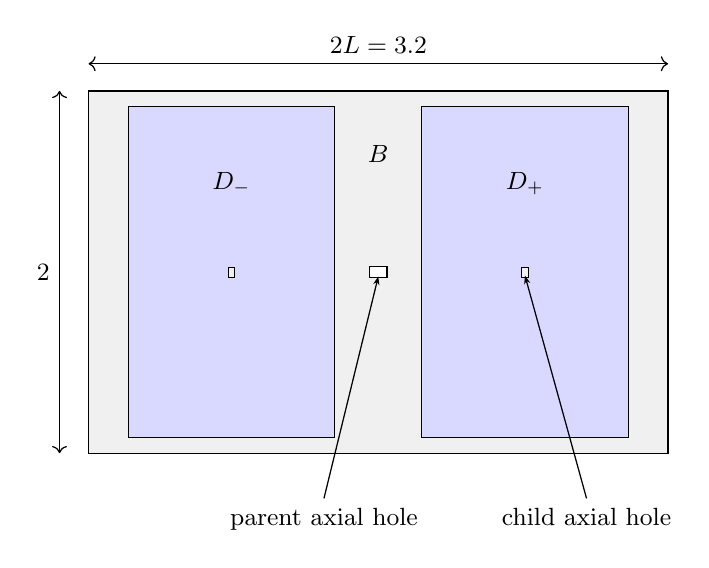
\begin{tikzpicture}[x=2.3cm,y=2.3cm,line width=0.45pt,
                    every node/.style={font=\small}]
 \filldraw[fill=black!6] (-1.6,-1) rectangle (1.6,1);
 \filldraw[fill=white] (-0.048,-0.03) rectangle (0.048,0.03);
 \filldraw[fill=blue!15] (-1.38,-0.912) rectangle (-0.24,0.912);
 \filldraw[fill=blue!15] (0.24,-0.912) rectangle (1.38,0.912);
 \filldraw[fill=black!6,line width=0.3pt]
   (-0.8271,-0.02736) rectangle (-0.7929,0.02736);
 \filldraw[fill=black!6,line width=0.3pt]
   (0.7929,-0.02736) rectangle (0.8271,0.02736);
 \node at (-0.81,0.49) {\(D_-\)};
 \node at (0.81,0.49) {\(D_+\)};
 \node at (0,0.65) {\(B\)};
 \draw[<->] (-1.6,1.15) -- (1.6,1.15)
   node[midway,above] {\(2L=3.2\)};
 \draw[<->] (-1.76,-1) -- (-1.76,1)
   node[midway,left] {\(2\)};
 \draw[-{Stealth[length=3pt]}] (-0.30,-1.25) -- (0,-0.025);
 \node[below,align=center] at (-0.30,-1.25)
   {parent axial hole};
 \draw[-{Stealth[length=3pt]}] (1.15,-1.25) -- (0.81,-0.02);
 \node[below,align=center] at (1.15,-1.25)
   {child axial hole};
\end{tikzpicture}
\caption{Top view of the cell geometry, at the exact planar scale.
The parent prism has \(\abs{x_3}<1\); the two shaded child prisms
have \(\abs{x_3}<s\). The small gray child holes belong to \(B\),
whereas the white central hole is outside \(D\). The available space
above and below the children connects the block.}
\label{nu:geometry-figure}
\end{figure}

Let \(\mu\) be the probability measure on \(\Sigma\) obtained
by pushing forward \((2\pi)^{-2}\dd\theta\,\dd\psi\) under
Equation~\eqref{nu:collar} at \(\tau=0\), and let
\(\mu_\pm=(S_\pm)_*\mu\). These measures have bounded positive
densities relative to surface measure on their respective fixed
boundaries. Apply Proposition~\ref{prop:branching-block} to \(B\)
with these three measures. We obtain a scalar conductivity
\(b\) and constants \(0<c_b\le C_b<\infty\) such that
\(c_b\le b\le C_b\) almost everywhere, with the exact property:
every \(b\)-harmonic field having separately constant boundary
voltages has conormal flux a constant multiple of the corresponding
probability measure on each component.

The ball \(\Omega\) strictly contains \(\overline D\), since the
parent outer box has maximal norm \(\sqrt{L^2+2}<3\).
For a finite word \(\nu\) over \(\{-,+\}\), let \(\abs\nu\)
denote its length, set \(S_\varnothing=\Id\), and define
\[
 S_{\nu\pm}=S_\nu\circ S_\pm,\qquad
 D_\nu=S_\nu D,\quad B_\nu=S_\nu B,\quad
 \Sigma_\nu=\partial D_\nu,\quad \mu_\nu=(S_\nu)_*\mu.
\]
Every \(S_\nu\) is a similarity of ratio \(s^{\abs\nu}\).
Its orthogonal part can reverse orientation, which does not affect
any scalar energy or change-of-variables formula. The sets \(B_\nu\)
are pairwise disjoint. Define
\begin{equation}\label{nu:gamma}
 \gamma(x)=
 \begin{cases}
  b(S_\nu^{-1}x),&x\in B_\nu\text{ for some }\nu,\\
  1,&\text{otherwise}.
 \end{cases}
\end{equation}
This is measurable and satisfies
\(c\le\gamma\le C\), where
\(c=\min(1,c_b)>0\) and \(C=\max(1,C_b)<\infty\).
The remaining nested set has volume zero, since the total volume of
the depth-\(j\) cells is
\begin{equation}\label{nu:null-set}
 2^j s^{3j}\abs D=(2s^3)^j\abs D\longrightarrow0,
 \qquad 2s^3=0.370386<1.
\end{equation}
The countably many boundary seams are also null sets. Their assigned
values in Equation~\eqref{nu:gamma} are immaterial.

\subsection{Surface charges and equal averages}

We first record both the exact source identity and its scaling.
For vectors in \(\R^3\), \(\abs p\) denotes Euclidean norm.

\Needspace{16\baselineskip}
\begin{lemma}\label{nu:source-lemma}
There is a constant \(K\), independent of \(\nu\), such that for
every \(p=(p_0,p_-,p_+)\) with \(p_0+p_-+p_+=0\), there exists
\(W_{\nu,p}\in H^1_0(\Omega)\cap L^\infty(\Omega)\), vanishing
off \(\overline{D_\nu}\) and constant on each child cell, with
\begin{equation}\label{nu:source-identity}
 \int_\Omega\gamma\nabla W_{\nu,p}\cdot\nabla\psi
 =p_0\int_{\Sigma_\nu}\operatorname{Tr}\psi\,\dd\mu_\nu
  +p_-\int_{\Sigma_{\nu-}}\operatorname{Tr}\psi\,\dd\mu_{\nu-}
  +p_+\int_{\Sigma_{\nu+}}\operatorname{Tr}\psi\,\dd\mu_{\nu+}
\end{equation}
for every \(\psi\in H^1(\Omega)\). It obeys
\begin{equation}\label{nu:source-bounds}
 \norm{W_{\nu,p}}_\infty\le K s^{-\abs\nu}\abs p,
 \qquad
 \int_\Omega\abs{\nabla W_{\nu,p}}^2
 \le K s^{-\abs\nu}\abs p^2.
\end{equation}
\end{lemma}

\begin{proof}
On the fixed block, let \(V=(V_0,V_-,V_+)\) be the constant voltage
vector and let \(p\) be the integrated outward conormal flux vector
of its harmonic extension \(v\). The map \(V\mapsto p\) is linear,
\(\sum_i p_i=0\), and
\[
 \int_B b\abs{\nabla v}^2=\sum_i V_i p_i.
\]
Thus its kernel consists exactly of common constants: zero flux implies
zero energy, and connectedness of \(B\) then makes \(v\) constant.
The induced map from voltage vectors modulo constants to zero-sum flux
vectors is an isomorphism of two-dimensional spaces. Normalize its
inverse by \(V_0=0\).

Extend \(v\) by \(V_\pm\) in \(D_\pm\) and by zero outside
\(\overline D\). Matching traces give an \(H^1\) function
\(W_p\) with compact support in \(\overline D\).
The exact block flux property gives Equation~\eqref{nu:source-identity}
at the root. This identity holds for every \(H^1\) test: equivalently,
one may first multiply the test by a smooth cutoff equal to one near
\(\overline D\). The boundary trace functionals are continuous,
since the measures have bounded surface densities. Invertibility of
the finite-dimensional map, the maximum principle for the bounded
boundary voltages, and the energy identity give
\[
 \norm{W_p}_\infty\le K\abs p,
 \qquad \int\abs{\nabla W_p}^2\le K\abs p^2.
\]

For \(j=\abs\nu\), set
\[
 W_{\nu,p}(x)=s^{-j}W_p(S_\nu^{-1}x),
\]
where \(W_p\) is understood to be zero outside \(\overline D\).
A similarity of ratio \(r\) multiplies energy and integrated flux
by \(r\) in dimension three when the scalar coefficient is copied
without changing its values. The extra voltage factor \(r^{-1}\),
here \(r=s^j\), therefore preserves the prescribed integrated
charges and gives the bounds in Equation~\eqref{nu:source-bounds}.
The coefficient inside the children is irrelevant because this
function has zero gradient there.
Finally,
\((S_\nu)_*\mu_\pm=\mu_{\nu\pm}\); hence the measure on each
shared boundary is exactly the same from its two adjacent blocks.
\end{proof}

\begin{lemma}\label{nu:equal-averages}
If \(u\in H^1(\Omega)\) is weakly \(\gamma\)-harmonic, then
\[
 m_\nu(u):=\int_{\Sigma_\nu}\operatorname{Tr}u\,\dd\mu_\nu
\]
has one common value \(u_*\) for all finite words \(\nu\).
If \(u\) is bounded, then \(\abs{u_*}\le\norm u_\infty\).
\end{lemma}

\begin{proof}
Test the weak equation for \(u\) with \(W_{\nu,p}\), and use
Equation~\eqref{nu:source-identity} with \(\psi=u\). This gives
\[
 p_0m_\nu(u)+p_-m_{\nu-}(u)+p_+m_{\nu+}(u)=0
 \qquad\text{whenever }p_0+p_-+p_+=0.
\]
The triple of averages is orthogonal to the zero-sum plane and is
therefore constant. Iterating proves the assertion. If \(u\) is
bounded, its traces have the same essential bounds: apply the trace
map to the vanishing positive-part truncations beyond those bounds.
Since every \(\mu_\nu\) is a probability measure, the last claim
follows.
\end{proof}

\subsection{A bounded potential carrying opposite limiting charges}

Give the two first-level cells charges \(q_-=1\) and \(q_+=-1\),
and recursively put \(q_{\nu-}=q_{\nu+}=q_\nu/2\). Thus
\begin{equation}\label{nu:charges}
 \abs{q_\nu}=2^{1-j}\quad(\abs\nu=j\ge1),
 \qquad \sum_{\abs\nu=j}\abs{q_\nu}=2.
\end{equation}
Define
\[
 Z_0=W_{\varnothing,(0,1,-1)},\qquad
 Z_j=\sum_{\abs\nu=j}
       W_{\nu,(-q_\nu,q_\nu/2,q_\nu/2)}\quad(j\ge1),
 \qquad
 w^{(N)}=\sum_{j=0}^{N-1}Z_j.
\]
The source identities telescope. For every integer \(N\ge1\) and
every \(\psi\in H^1(\Omega)\),
\begin{equation}\label{nu:finite-source}
 \int_\Omega\gamma\nabla w^{(N)}\cdot\nabla\psi
 =\sum_{\abs\nu=N}q_\nu
      \int_{\Sigma_\nu}\operatorname{Tr}\psi\,\dd\mu_\nu.
\end{equation}

\begin{lemma}\label{nu:potential}
The sequence \(w^{(N)}\) converges in both \(L^\infty(\Omega)\)
and \(H^1(\Omega)\) to a nonzero
\(w\in H^1_0(\Omega)\cap L^\infty(\Omega)\) that vanishes
almost everywhere off \(\overline D\).
\end{lemma}

\begin{proof}
At a fixed depth the cell interiors are disjoint. Combining
Equations~\eqref{nu:source-bounds} and~\eqref{nu:charges}, with a
larger constant \(K\) if necessary, gives
\begin{equation}\label{nu:level-bounds}
 \norm{Z_j}_\infty\le K(2s)^{-j},\qquad
 \norm{\nabla Z_j}_2^2\le K(2s)^{-j}.
\end{equation}
Since \(2s=1.14>1\), both
\(\sum_j\norm{Z_j}_\infty\) and
\(\sum_j\norm{\nabla Z_j}_2\) converge. The first controls the
\(L^2\) norms as well because \(\Omega\) is bounded. This proves
the asserted convergence. Every partial sum is in \(H^1_0(\Omega)\)
and vanishes off \(\overline D\); the same is true of its limit.

To show that \(w\ne0\), fix
\(\eta\in C_c^\infty(\Omega)\) equal to one on a neighborhood
of \(\overline{D_-}\) and zero on a neighborhood of
\(\overline{D_+}\). The positive separation of these compact sets
makes this possible. At every depth the signed total in the first
left cell is \(1\) and that in the first right cell is \(-1\).
Equation~\eqref{nu:finite-source} therefore gives
\[
 \int_\Omega\gamma\nabla w^{(N)}\cdot\nabla\eta=1.
\]
Strong \(H^1\) convergence yields
\begin{equation}\label{nu:nonzero}
 \int_\Omega\gamma\nabla w\cdot\nabla\eta=1,
\end{equation}
which proves nontriviality. No trace or pointwise value on the limiting
nested set has been used.
\end{proof}

\subsection{An exact transformation of all boundary measurements}

The transformation in this subsection is related to the conformal
energy identity used by Daud\'e, Kamran, and
Nicoleau~\cite[Proposition~1.2]{DaudeKamranNicoleau}.
Here Equation~\eqref{nu:nonzero} shows that $w$ has a nonzero source.
The decisive property is that this source vanishes on every product
$(u-u_*)\phi$ with $u$ bounded and harmonic and $\phi$ a smooth compactly
supported test. We prove that identity before transforming the
harmonic extensions.

Choose a real \(\delta\ne0\) such that
\(\abs\delta\norm w_\infty<1/2\), and set
\begin{equation}\label{nu:new-coefficient}
 \rho=1+\delta w,\qquad \widetilde\gamma=\rho^2\gamma.
\end{equation}
Then
\begin{equation}\label{nu:ellipticity}
 \tfrac12\le\rho\le\tfrac32,
 \qquad \tfrac c4\le\widetilde\gamma\le\tfrac{9C}4
 \quad\text{almost everywhere}.
\end{equation}
Both conductivities equal one in a neighborhood of \(\partial\Omega\).
They differ on a set of positive measure: by
Equation~\eqref{nu:nonzero}, \(w\) is not zero almost everywhere,
and positivity of \(\rho\) makes \(\rho^2=1\) equivalent to
\(w=0\).

\begin{lemma}\label{nu:weighted-identity}
Let \(u\) be a bounded weakly \(\gamma\)-harmonic function in
\(\Omega\), and let \(u_*\) be its common average from
Lemma~\ref{nu:equal-averages}. Then, for every
\(\phi\in C_c^\infty(\Omega)\),
\begin{equation}\label{nu:weighted}
 \int_\Omega\gamma\nabla\rho\cdot
       \nabla\bigl((u-u_*)\phi\bigr)=0.
\end{equation}
\end{lemma}

\begin{proof}
The product \((u-u_*)\phi\) belongs to \(H^1_0(\Omega)\),
so it is an admissible test in Equation~\eqref{nu:finite-source}.
Put \(M=\norm u_\infty\). For each depth-\(N\) cell choose
\(x_\nu\in\overline{D_\nu}\). The zero-average identity on its
surface gives
\[
 \int_{\Sigma_\nu}(\operatorname{Tr}u-u_*)\phi\,\dd\mu_\nu
 =\int_{\Sigma_\nu}(\operatorname{Tr}u-u_*)
       \bigl(\phi-\phi(x_\nu)\bigr)\,\dd\mu_\nu.
\]
Since \(\abs{\operatorname{Tr}u-u_*}\le2M\) almost everywhere on this surface,
the absolute value of the sum on the right-hand side of
Equation~\eqref{nu:finite-source} is at most
\begin{equation}\label{nu:diameter-error}
 4M\norm{\nabla\phi}_\infty\,\operatorname{diam}(D)\,s^N.
\end{equation}
Here we used Equation~\eqref{nu:charges} and
\(\operatorname{diam}(D_\nu)=s^N\operatorname{diam}(D)\).
This tends to zero. The fixed product test has square-integrable
gradient, so strong \(H^1\) convergence of \(w^{(N)}\), together
with boundedness of \(\gamma\), justifies passage to the limit on
the left. Multiplication by \(\delta\) proves
Equation~\eqref{nu:weighted}.
\end{proof}

\begin{proposition}\label{nu:identical-dn}
The full weak Dirichlet-to-Neumann operators of \(\gamma\) and
\(\widetilde\gamma\) on \(\Omega\) are equal.
\end{proposition}

\begin{proof}
First take \(f\in C^\infty(\partial\Omega)\), and let \(u\)
be its weak \(\gamma\)-harmonic extension. The weak maximum
principle, obtained by testing truncations beyond the boundary bounds,
gives \(\norm u_\infty\le\norm f_\infty\). Define
\begin{equation}\label{nu:transformed-solution}
 \widetilde u=u_*+\frac{u-u_*}{\rho}.
\end{equation}
The Sobolev chain rule applies to \(1/\rho\) on the interval
\([1/2,3/2]\), and the product rule applies because both factors
are bounded \(H^1\) functions. Hence \(\widetilde u\in H^1(\Omega)\),
and it equals \(u\) off \(\overline D\), in particular near
the outer boundary. Its flux is
\begin{equation}\label{nu:transformed-flux}
 \widetilde\gamma\nabla\widetilde u
 =\rho\gamma\nabla u-(u-u_*)\gamma\nabla\rho.
\end{equation}
This is an \(L^2\) vector field.

For \(\phi\in C_c^\infty(\Omega)\), use \(\rho\phi\in H^1_0(\Omega)\)
in the original weak equation to obtain
\[
 \int_\Omega\rho\gamma\nabla u\cdot\nabla\phi
 =-\int_\Omega\phi\gamma\nabla u\cdot\nabla\rho.
\]
Equation~\eqref{nu:weighted}, expanded by the product rule, also gives
\[
 \int_\Omega(u-u_*)\gamma\nabla\rho\cdot\nabla\phi
 =-\int_\Omega\phi\gamma\nabla\rho\cdot\nabla u.
\]
Subtracting proves that the divergence of the flux in
Equation~\eqref{nu:transformed-flux} is zero. All cross-gradient
products are integrable by Cauchy--Schwarz; boundedness of the other
factors also gives the stated \(L^2\) flux bound. Density of smooth
tests in \(H^1_0(\Omega)\) proves the full weak equation.
By uniqueness, \(\widetilde u\) is the
\(\widetilde\gamma\)-harmonic extension of \(f\).

Now fix arbitrary \(g\in H^{1/2}(\partial\Omega)\) and choose
an \(H^1\) extension \(V\) of \(g\). Multiply \(V\) by a smooth
cutoff that equals one near \(\partial\Omega\) and is supported
in an outer collar disjoint from \(\overline D\). The resulting
\(V_0\) still has trace \(g\), and its gradient is supported
where the two solution fluxes agree. Consequently the defining weak
pairings satisfy
\[
 \langle\Lambda_{\widetilde\gamma}f,g\rangle
 =\int_\Omega\widetilde\gamma\nabla\widetilde u\cdot\nabla V_0
 =\int_\Omega\gamma\nabla u\cdot\nabla V_0
 =\langle\Lambda_\gamma f,g\rangle.
\]
Both operators are bounded from \(H^{1/2}\) to \(H^{-1/2}\) by
the elliptic energy estimate. Since smooth boundary functions are
dense in \(H^{1/2}(\partial\Omega)\) on the ball, equality extends
from smooth \(f\) to all boundary traces. This last step does not
require extending the transformation in
Equation~\eqref{nu:transformed-solution} to unbounded solutions.
\end{proof}

\begin{proof}[Proof of Theorem~\ref{thm:main}]
Lemma~\ref{nu:geometry} permits the use of
Proposition~\ref{prop:branching-block}, and
Equation~\eqref{nu:gamma} constructs a uniformly positive bounded
scalar conductivity on the ball \(\Omega=B(0,3)\subset\R^3\).
Lemmas~\ref{nu:source-lemma}--\ref{nu:potential} produce the bounded
nonzero function used in Equation~\eqref{nu:new-coefficient}.
The second scalar conductivity has the positive bounds in
Equation~\eqref{nu:ellipticity}, agrees with the first near the
boundary, and differs from it on a set of positive measure.
Set $\gamma_0=\gamma$ and $\gamma_1=\widetilde\gamma$, with common
positive finite bounds obtained by taking the smaller lower bound
and the larger upper bound. Proposition~\ref{nu:identical-dn} proves
equality of their full weak Dirichlet-to-Neumann operators. Thus
these coefficients give the
claimed counterexample in dimension three, disproving the assertion
quantified over all \(n\ge3\).
\end{proof}

\begin{proof}[Proof of Corollary~\ref{cor:localized}]
Return to the notation of Corollary~\ref{cor:localized}: let $\Omega$
be its bounded connected Lipschitz domain, let $c,C$ be the common bounds
from Theorem~\ref{thm:main}, and let $B_1,\ldots,B_m$ be the prescribed balls.
Write $B_i=B(x_i,r_i)$ and set $U_i=B(x_i,r_i/2)$.
The closed balls $\overline U_i$ are separated from one another and
from $\partial\Omega$, even if some prescribed balls have tangent
boundaries. Let $a_0,a_1$ be the pair of Theorem~\ref{thm:main},
and put $\Phi_i(y)=x_i+s_i y$, where $s_i=r_i/6$.
This maps $B(0,3)$ onto $U_i$. Copy the scalar coefficients by
composition: $a_{i,j}=a_j\circ\Phi_i^{-1}$ on $U_i$.
If $q_{i,j}(h)$ is the minimum energy with trace
$h\in H^{1/2}(\partial U_i)$, change of variables gives
\[
 q_{i,j}(h)=s_i
 \ip{\Lambda_{a_j}(h\circ\Phi_i)}{h\circ\Phi_i}.
\]
Thus $q_{i,0}=q_{i,1}$. The coefficient values and their unit
boundary collars are preserved; no amplitude rescaling is needed.

Define $\gamma_\varepsilon=a_{i,\varepsilon_i}$ on $U_i$ and
$\gamma_\varepsilon=1$ elsewhere. The stated bounds follow because
the original unit collars imply $c\leq1\leq C$.
Let $E=\Omega\setminus\bigcup_i\overline U_i$, and denote by
$E_{\rm ext}(f,h_1,\ldots,h_m)$ the minimum unit-conductivity
energy on $E$ with outer trace $f$ and inner traces $h_i$.
The trace theorem and matching-trace $H^1$ gluing, together with
Equation~\eqref{eq:energy-minimum}, give
\[
 \ip{\Lambda_{\gamma_\varepsilon}f}{f}
 =\min_{h_i\in H^{1/2}(\partial U_i)}
 \left\{E_{\rm ext}(f,h_1,\ldots,h_m)
       +\sum_{i=1}^m q_{i,\varepsilon_i}(h_i)\right\}
 \qquad(f\in H^{1/2}(\partial\Omega)).
\]
Indeed, restriction of a global competitor gives one inequality,
and gluing the subdomain minimizers gives the other; a global
minimizer supplies an attaining tuple of interface traces.
The right side is independent of $\varepsilon$. Polarization
therefore proves equality of the full weak operators.

If two indices differ at position $i$, their conductivities differ
inside $U_i$ on a set of measure
$s_i^3\abs{\{a_0\ne a_1\}}>0$. This proves all $2^m$ choices
are distinct. Their common boundary response is not asserted to be
that of the constant conductivity one.
\end{proof}

\Needspace{30\baselineskip}
\begingroup
\raggedright
\begin{thebibliography}{99}

\bibitem{AstalaFaracoSzekelyhidi}
K.~Astala, D.~Faraco, and L.~Sz\'ekelyhidi, Jr.,
Convex integration and the $L^p$ theory of elliptic equations,
\emph{Annali della Scuola Normale Superiore di Pisa,
Classe di Scienze} (5) \textbf{7} (2008), no.~1, 1--50.
\href{https://www.numdam.org/item/ASNSP_2008_5_7_1_1_0/}
{Numdam: ASNSP\_2008\_5\_7\_1\_1\_0}.

\bibitem{AstalaPaivarinta}
K.~Astala and L.~P\"aiv\"arinta,
Calder\'on's inverse conductivity problem in the plane,
\emph{Annals of Mathematics} (2) \textbf{163} (2006), no.~1, 265--299.
\href{https://doi.org/10.4007/annals.2006.163.265}
{doi:10.4007/annals.2006.163.265}.

\bibitem{Calderon}
A.~P.~Calder\'on,
On an inverse boundary value problem,
in \emph{Seminar on Numerical Analysis and its Applications to Continuum
Physics}, Sociedade Brasileira de Matem\'atica, Rio de Janeiro, 1980,
pp.~65--73.
Reprinted in \emph{Computational and Applied Mathematics}
\textbf{25} (2006), no.~2--3, 133--138.
\href{https://doi.org/10.1590/S0101-82052006000200002}
{doi:10.1590/S0101-82052006000200002}.

\bibitem{CaroRogers}
P.~Caro and K.~M.~Rogers,
Global uniqueness for the Calder\'on problem with Lipschitz
conductivities,
\emph{Forum of Mathematics, Pi} \textbf{4} (2016), e2.
\href{https://doi.org/10.1017/fmp.2015.9}{doi:10.1017/fmp.2015.9}.

\bibitem{DaudeKamranNicoleau}
T.~Daud\'e, N.~Kamran, and F.~Nicoleau,
On nonuniqueness for the anisotropic Calder\'on problem with partial data,
\emph{Forum of Mathematics, Sigma} \textbf{8} (2020), e7.
\href{https://doi.org/10.1017/fms.2020.1}{doi:10.1017/fms.2020.1}.

\bibitem{Haberman}
B.~Haberman,
Uniqueness in Calder\'on's problem for conductivities with unbounded
gradient,
\emph{Communications in Mathematical Physics}
\textbf{340} (2015), no.~2, 639--659.
\href{https://doi.org/10.1007/s00220-015-2460-3}
{doi:10.1007/s00220-015-2460-3}.

\bibitem{Kirchheim}
B.~Kirchheim,
\emph{Rigidity and Geometry of Microstructures},
habilitation thesis, Universit\"at Leipzig, 2003;
Lecture Note 16/2003, Max Planck Institute for Mathematics in the Sciences.
\href{https://www.mis.mpg.de/publications/preprint-repository/lecture_note/2003/issue-16}
{MPI MIS Lecture Note 16/2003}.

\bibitem{MarinoSpagnolo}
A.~Marino and S.~Spagnolo,
Un tipo di approssimazione dell'operatore
$\sum_{i,j=1}^{n}D_i(a_{ij}(x)D_j)$ con operatori
$\sum_{j=1}^{n}D_j(\beta(x)D_j)$,
\emph{Annali della Scuola Normale Superiore di Pisa,
Classe di Scienze} (3) \textbf{23} (1969), no.~4, 657--673.
\href{https://www.numdam.org/item/ASNSP_1969_3_23_4_657_0/}
{Numdam: ASNSP\_1969\_3\_23\_4\_657\_0}.

\bibitem{Miller}
K.~Miller,
Nonunique continuation for uniformly parabolic and elliptic equations
in self-adjoint divergence form with H\"older continuous coefficients,
\emph{Archive for Rational Mechanics and Analysis}
\textbf{54} (1974), no.~2, 105--117.
\href{https://doi.org/10.1007/BF00247634}{doi:10.1007/BF00247634}.

\bibitem{OpenAISmoothPatch2026}
OpenAI,
Smooth anisotropic uniqueness in the Calder\'on problem from one boundary patch,
OpenAI Math Release preprint
\href{https://github.com/openai/math/blob/main/preprints/Smooth-Anisotropic-Uniqueness-in-the-Calderon-Problem-from-One-Boundary-Patch-September-24-2026/paper.pdf}{OAI:Smooth-Anisotropic-Uniqueness-in-the-Calderon-Problem-from-One-Boundary-Patch-September-24-2026},
2026.

\bibitem{Raita}
B.~Rai\textcommabelow{t}\u a,
Potentials for $\mathcal A$-quasiconvexity,
\emph{Calculus of Variations and Partial Differential Equations}
\textbf{58} (2019), article 105.
\href{https://doi.org/10.1007/s00526-019-1544-x}
{doi:10.1007/s00526-019-1544-x}.

\bibitem{Rondi}
L.~Rondi,
Continuity properties of Neumann-to-Dirichlet maps with respect to
the $H$-convergence of the coefficient matrices,
\emph{Inverse Problems} \textbf{31} (2015), no.~4, 045002.
\href{https://doi.org/10.1088/0266-5611/31/4/045002}
{doi:10.1088/0266-5611/31/4/045002}.

\bibitem{SylvesterUhlmann}
J.~Sylvester and G.~Uhlmann,
A global uniqueness theorem for an inverse boundary value problem,
\emph{Annals of Mathematics} (2) \textbf{125} (1987), no.~1, 153--169.
\href{https://doi.org/10.2307/1971291}{doi:10.2307/1971291}.

\end{thebibliography}

\endgroup
\end{document}
